\documentclass[10pt,hidelinks]{article}

\usepackage[margin=0.75in,top=0.75in,footskip=0.5in]{geometry}
\usepackage{comment}
\usepackage{helvet}
\renewcommand{\familydefault}{\sfdefault}
% use Unicode characters - try changing the option if you run into troubles with special characters (e.g. umlauts)
\usepackage[utf8]{inputenc}
% clean citations
\usepackage{cite}
% hyperref makes references clicky. use \url{www.example.com} or \href{www.example.com}{description} to add a clicky url
\usepackage{nameref,hyperref}
% line numbers
%\usepackage[right]{lineno}
% improves typesetting in LaTeX
\usepackage{microtype}
\DisableLigatures[f]{encoding = *, family = * }
% Remove % for double line spacing
%\usepackage{setspace} 
%\doublespacing

% use adjustwidth environment to exceed text width (see examples in text)
\usepackage{changepage}
% use \textcolor{color}{text} for colored text (e.g. highlight to-do areas)
\usepackage{color}
% this is required to include graphics
\usepackage{graphicx}
% use for have text wrap around figures
\usepackage{wrapfig}
\usepackage{setspace}
%\doublespacing
\usepackage{multicol}
\usepackage{enumitem}
\usepackage{caption}
\captionsetup[figure]{font=footnotesize,skip=0pt}
\usepackage{subcaption} 
\usepackage{authblk}
\usepackage{indentfirst}

\newcommand{\beginsupplement}{%
        \setcounter{table}{0}
        \renewcommand{\thetable}{S\arabic{table}}%
        \setcounter{figure}{0}
        \renewcommand{\thefigure}{S\arabic{figure}}%
     }
\newcommand{\gp}[]{\textsc{gp }}
%%%%%%%%%%%%%% TITLE 
%Title: Should not exceed 25 words and should be specific and informative. Trade marks and proprietary terms are not allowed in the title.


%Running title: Should not exceed 50 characters.

%Authors: Give initials and family name of all authors.

%(Please refer to the section ‘To accompany manuscript at submission’ for more details regarding authorship entitlements)
%NB - A declaration of Author’s roles is required at submission and this information MUST be included in the manuscript (after the discussion, before the Acknowledgements).
%Author affiliations and addresses: The department, institution, city and country should be given with postal code for each author. An e mail address will be published for the corresponding author, who should be clearly identified with an asterisk. Current addresses should be provided for all authors.

% title goes here:
\title{Prioritization of putatively detrimental variants in euploid miscarriages}
%Running title: Should not exceed 50 characters.
\author[1+]{Silvia Buonaiuto}
\author[2+]{Imma Di Biase}
\author[3]{Valentina Aleotti}
\author[3]{Amin Ravaei}
\author[4]{Adriano De Marino}
\author[1]{Gianluca Damaggio}
\author[5]{Marco Chierici}
\author[6]{Madhuri Pulijala}
\author[2]{Palmira D’Ambrosio} 
\author[2]{Gabriella Esposito}
\author[6,7]{Qasim Ayub}
\author[8]{Cesare Furlanello}
\author[9]{Pantaleo Greco}
\author[4]{Antonio Capalbo}
\author[3]{Michele Rubini}
\author[2]{Sebastiano Di Biase}
\author[1*]{Vincenza Colonna}
%\author[]{{\color{blue} nomi memorial exomes} }
\affil[1]{Institute of Genetics and Biophysics, National Research Council, Naples, 80111, Italy}
\affil[2]{MeriGen Research, Naples, 80131, Italy}
\affil[3]{Department of Neurosciences and Rehabilitation, University of Ferrara, Ferrara, 44121, Italy.}
\affil[4]{Igenomix Italy, Marostica, 36063, Italy}
\affil[5]{Fondazione Bruno Kessler, MPBA Lab, Trento, 38123, Italy}
\affil[6]{Monash University Malaysia Genomics Facility, Tropical Medicine and Biology Multidisciplinary Platform, 47500 Bandar Sunway, Malaysia.}
\affil[7]{School of Science, Monash University Malaysia, 47500 Bandar Sunway, Malaysia.}
\affil[8]{HK3 Lab, Rovereto,38068, Italy}
\affil[9]{Department of Medical Sciences, University of Ferrara, Ferrara, 44121,Italy.}
\affil[*]{Correspondence: vincenza.colonna@igb.cnr.it}
\affil[+]{these authors contributed equally to this work}
\setcounter{Maxaffil}{0}
\renewcommand\Affilfont{\itshape\small}
\date{}

%%%%%%%%%%%%%%%%%%%%%%%%%%%%%%%%%%%%%%%%%%%%%%%%%%%%%%%%%%%%%%%%%%%%%%%%%%%%
% document begins here
\begin{document}
\maketitle
\newpage
\section*{Abstract}

%All original research articles published in Human Reproduction are now required to have an extended abstract. The aim behind the change to this new format is to capture the essence, novelty and importance of each study, making the information more instantly available to readers. The abstract should clearly set out the research question, study design, findings, implications, funding and competing interests.

%Use MESH* terms in title and abstract.
%* for MESH terms see PubMed at http://www.ncbi.nlm.nih.gov/pubmed/
%Version 2.6     25/01/2013

%Please complete all sections; please do not remove or change headings.

%\subsection*{\textsc{Title}} add title and uncomment if abstract is sent separately 
%[if randomised, identify the study as such in title]

\subsection*{\textsc{Study question:}} 
%[A SINGLE question (ending in a question mark), limited to the PRIMARY objective of the study ONLY (do not include secondary questions)]
Do prioritization of genomic variants based on their functional features informs on genes putatively causative and clarify the impact of small-size genetic variants in the study of genome of euploid embryos from pregnancy losses? (SPECIFICO)  

OPPURE 

Do the analysis of genome sequences of euploid embryos from pregnancy loss informs on genes putatively causative of the miscarriage and clarify the impact of small-size genetic variants? (GENERICO) 

%Miscarriages are frequent events with a complex aetiology whose genetic components have not been completely understood. We developed a scalable pipeline that investigates genetic variation scantily considered in the context of miscarriages. We use our pipeline to analyze coding regions of the genome of ten miscarried euploid embryos to prioritize putatively detrimental variants in genes that are relevant for embryonic development.

\subsection*{\textsc{Summary answer:}}  
%[The main conclusion. A single sentence, this should be limited to the primary results of the study, without any discussion of their implications]
Filtering and prioritizing genetic variants is effective in identifying genomic variants putatively responsible for miscarriages. 

\subsection*{\textsc{What is known already:}} 
%[One or two short sentences] 
%100 Pregnancy Loss (PL), the spontaneous demise of a pregnancy before 24 weeks of gestation, occurs in 10-15\% of pregnancies. 
Miscarriage is often the result of chromosomal aneuploidies of the gametes but it can also have non random genetic causes like small-size mutations, both \textit{de novo} or inherited from parents, that have been scantily investigated so far. Analysis of genomic sequences of miscarried embryos has been mostly focusing on rare variation, and carried out using quite non homogeneous criteria and methods that are difficult to reproduce. 

\subsection*{\textsc{Study design, size, duration:}} 
%[Cross sectional – control versus treatment, longitudinal –time-course, age-course. Numbers of treated/controls, treatment duration, sampling procedures]
This is a monocentric observational study. The study includes the data analysis of 46 embryos obtained from women experiencing pregnancy loss recruited by the University of Ferrara from 2017 to 2018. The study was approved by the Ethical committee of Emilia-Romagna CE/FE #170475. 
 
\subsection*{\textsc{Participants/materials, setting, methods:}} %[General approach used eg cell/tissue culture/transfection, animal treatments/models, transgenesis. Species, ages, gender, cell type. Methods and endpoints used – eg hormone, cytokine, growth factor measurements, cell numbers/proliferation, tissue morphology/composition, FACS, immunohistochemistry, Westerns, quantitative PCR, FISH]
Participants are forty-six women, mostly European (87\%) diagnosed with first (n=25, av.age 32.7 ) or recurrent (n=21, av.age 36.5) miscarriage. Embryonic DNA was prepared form chorionic villi and used to select euploid embryos using quantitative PCR, comparative genomic hybridiztion and shallow sequencing of random genomic regions. Euploid embryos were whole-genome sequenced at 30X using Illumina short reads technology and genomic sequences used to identify genetic variants. Variants were annotated integrating information from Ensembl100 and literature knowledge on genes associated with embryonic development, miscarriages, lethality, cell cycle. Following annotation, variants were filtered to prioritize putatively detrimental variants in genes that are relevant for embryonic development using a pipeline that we developed. The code is available on gitHub (ezcn/grep).

\subsection*{\textsc{Main results and the role of chance:}} 
%[P values, biological gradient, repeatability/robustness, mechanisms identified/involved]
Our pipeline prioritized 439 putatively causative single nucleotide polymorphisms among 11M variants discovered in ten embryos. Systematic investigation of all coding regions selected about 47 genes per embryo. Among them \textit{STAG2}, known in literature for its role in congenital and developmental disorders as well as in cancer, \textit{TLE4} a key gene in embryonic development, expressed in both embryonic and extraembryonic tissues in the Wnt and Notch signalling pathways, and \textit{FMNL2}, involved in cell motility with a major role in driving cell migration. Our results are fully reproducible (the code is open-source) and robust, as we exclude genes with $>$5\% chance to be selected in a control population.  

\subsection*{\textsc{Limitations, reasons for caution:}} 
%[Descriptive, only in vitro, cell transfection, shown only in one species, technical limitations and reasons for caution, cell/animal lethality in a knock-out, disease- or cell-specificity]
Despite producing encouraging results, this pilot study has major limitations in sample size and lack of integration of the parental genomic information. %

\subsection*{\textsc{Wider implications of the findings :}} 
%[Agreement/disagreement with literature, resolution of previous disparity, new insights/mechanisms in disease(s), new therapeutic potential, cell-, species- gender-, or age-implications, relevance to other systems]
This pilot study demonstrate that analysis of genome sequencing can help to clarify the causes of idiopathic miscarriages and provides initial results from the analysis of ten euploid embryos. We discovered plausible candidate genes and variants and provides essential indications to scale to a larger study. Results of this and following wider studies can be used to test genetic predisposition to miscarriages in parents that are planning to conceive or in preimplantation genetic testing. In a more wide context, results of this study might be relevant for genetic counseling and risk management in miscarriages

\subsection*{\textsc{Study funding/competing interest(s):}} %Trial registration number: a trial registration number is only required for clinical trials.


\section*{Key words}
%Up to ten key words must be supplied by the author. The key words, together with the title and abstract, are used for online searches. They should therefore be specific and relevant to the paper.

miscarriage, embryos, whole-genome sequencing, variant prioritization, genetic of infertility, embryo aneuploidies, infertility diagnosis, \textit{TLE4}, \textit{STAG2}, \textit{FMNL2}

%%%%%%%%%%%%%%%%%%%%%%%
%The introduction should be limited to the specific background necessary to show the importance and context of the current study. The objective of the study should be clearly stated in the final paragraph of the Introduction.

\section*{Introduction}
%Indicate the field of the work, why this field is important, and what has already been done (with proper citations).
%Indicate a gap, raise a research question, or challenge prior work in this territory.
%outline the purpose and announce the present research, clearly indicating what is novel and why it is significant.
%avoid: repeating the abstract; providing unnecessary background information; exaggerating the importance of the work; claiming novelty without a proper literature search. 

%%%%%%%%%%%%%%%%%• Present the problem and the proposed solution %%%%%%%%%%%%%%%%%• Presents nature and scope of the problem investigated
Miscarriage, i.e. the spontaneous termination of a pregnancy before 24 weeks of gestation, occurs in  10-15\% of all pregnancies \cite{larsen2013new,ammon2012systematic, andersen2000maternal} and has both environmental and genetic causes\cite{larsen2013new}. Miscarriages are often the result of chromosomal aneuploidies of the gametes but they can also have non random genetic causes like small mutations (SNPs and indels), both de-novo or inherited from parents. Miscarriages are mostly studied using parental genetic information \cite{pereza2017systematic} and at a resolution that leaves unexplored the vast majority of the genome. Comparative genomic hybridization detects variants of several thousand base pairs \cite{robberecht2009diagnosis, kudesia2014rescue,mathur2014miscarriage} while targeted resequencing resolves point mutations. Both are currently the most accurate methods for the genetic analysis of parental DNA of miscarriages but are not sensitive to small variants, or target only a few coding regions. On a different approach, the only study so far that tests for genome-wide genetic association in a large cohort of miscarriages is also based on maternal information \cite{laisk2020genetic}. Depending on the mode of inheritance the study of parental genome might be ineffective as it will reveal only half of the inheritance that was effectively passed to the embryo and it would miss \textit{de novo} mutations. Extending therefore the analysis to fetal genomes is the necessary next step to fully understand the genetics of miscarriages with an approach that systematically targets also small-size genetic variants. 
%The incidence of genomic abnormalities in RPL is estimated to be around 50\% \cite{van2012genetics}. 

%%%%%%%%%%%%%%%%% • Reviews the pertinent literature to orient the reader
%%literature: miscarriages sequences 
DNA sequence information of miscarried fetuses has been already used to determine the genetic component of miscarriages in some studies\cite{rajcan2020next, filges2015exome}. Most studies adopt a family-based approach often with focus on a reduced range of fetal phenotype, integrating pedigree and parental genomic data\cite{bondeson2017nonsense, dohrn2015ecel1,wilbe2015musk, cristofoli2017novel}.Some among those focusing only on embryos target candidates genes. Examples are the identification of a mutation in the X-linked gene \textit{FOXP3} in siblings male miscarriages \cite{rae2015novel}, and the identification of a truncating \textit{TCTN3} mutations in unrelated embryos\cite{thomas2012tctn3}. A number of studies focuse instead on exome sequences\cite{shamseldin2015identification, qiao2016whole,fu2018whole, meier2019exome, yates2017whole}. One study selects only variants transmitted to both sibling miscarriages \cite{qiao2016whole}, others limit to autozygous variants\cite{thomas2012tctn3, shamseldin2015identification}, some focus on delivering accurate diagnosis \cite{meier2019exome}. All these studies consider number of cases in the order of the tens and in most cases are motivated by phenotypic information mostly deriving from ultrasound scans. 
%%%%%%%%%%%%%focus in idiopathic 
Two other studies adopt a cohort-based approach analyzing up to thousands of embryonic genomes with a range of phenotypes\cite{chen2017characterization,zhao2020exome}. One of them focuses on  searching causative variants, demonstrating that exome sequencing effectively informs genetic diagnosis in about one-third of the 102 cases considered\cite{zhao2020exome}. The other one focuses on conserved genes in copy number variable (CNV) regions in 1810 cases to identify 275 genes, often in clusters, located in the CNVs and potentially implicated essential embryonic developmental processes\cite{chen2017characterization}.
%%literature: prioritization pipelines 
Because the number of embryos is always small for genetic association analysis to be effective, all studies mentioned so far perform sequencing followed by variant annotation and prioritization. All investigate supposedly euploid embryos and focus on rare variation, nevertheless always using different criteria to select the variants and never releasing code to fully reproduce the variant prioritization making difficult to replicate results and perform comparisons.  
%\cite{qiao2016whole}software non opensource no popcomparison  no overlap genes 
%TRAPD  286 selected candidate genes\FU2018 looking only for candidate genes bias 
%poor overlap with results   % apart from TRAPD, no scripts available 


%%%%%%%%%%%%%%%%%• States the method of the experiment
In this study, we performed whole-genome sequencing on euploid embryos from idiopathic spontaneous pregnancy losses and developed \gp, a pipeline to prioritize putatively causative variants. As first step \gp performs filtering of high-quality genomic variants based on prediction of the functional effect of the variants and using a set of parameters that can be specified by the user. This first selection is completed by filters for technical artifacts (e.g. mapping errors, read depth) and a filter for random selection of genes in a control cohort through resampling. Our pipeline can incorporate prior information on candidate genes, and is also robust to the discovery of novel genes.  %Finally, it is possible to test if the frequency of the selected variants is compare the frq  
%%%%%%%%%%%%%%%%%• State the principle results of the experiment 
We prioritize on average 49 variants per embryo with high and moderate impact in genes relevant for embryonic development and mitochondrial metabolism, some of which were previously identified for having a role in miscarriages. We demonstrate that variant prioritization can be already effective when dealing with a limited number of samples. This preliminary study will facilitate the development of a larger-scale project to inform molecular diagnosis of pregnancy loss. 



%Human reproduction is highly ineffective and it is estimated that 10-20\% of all pregnancies end in early miscarriage or early pregnancy loss (PL) during the first trimester [REF SILVIA] and up to 50\% of cases of RPL do not have a clearly defined etiology\cite{practice2012evaluation}. Miscarriage is defined as the death of the fetus within 20-28 week of gestation\cite{pmid27994187, pmid25055407, pmid25944391, pmid11821293, stephenson2002cytogenetic, pmid25681385, pmid29858908}. Recurrent pregnancy loss (RPL) is defined as the loss of two or more consecutive pregnancies\cite{green2019review}. RPL has a high impact on public health since it affects up to 3-5\% of couples[REF PER QUESTO]. For 50-60\% of RPL cases the cause are known to be structural genetic, endocrine, anatomic, thrombophilic, autoimmune, and environmental factors, however for the remaining 40-50\% the causes are unknown\cite{pmid27994187, pmid25944391, pmid11821293, stephenson2002cytogenetic, pmid22796359, pmid22672580, pmid25681385, gaboon2013recurrent, pmid30642578}.\\


%The diagnosis of miscarriages is based on embryo heart activity and gestational sac features revealed by ultrasonography\cite{doubilet2013diagnostic}. Nevertheless, diagnosis take place only after the death of the embryo, and only few cases there are followed-up to understand the genetic causes with techniques that can discriminate anouplidies (kariotyping, quantitative PCR) or large deleterious copy number variants (comparative genomic hybridization), while no information is available on small-size DNA changes incompatible with life. Therefore, the current ability of inform prognosis and manage decision in cases of perinatal lethality is limited, with important consequences in counseling for RPLs and \textit{in-vitro} fertilization.\\

%Among PL caused by genetic defects, it is estimated that 50-70\% [check PERCENT] is due to meiotic chromosome segregation errors, whose frquency increases with increasing maternal age\cite{pmid30393965, pmid10864550, pmid20041396}. Sperm DNA fragmentation caused by oxidative stress also causes PL through impairment of placentation \cite{pmid2972074, pmid30448091, pmid30602480}. %as well as increased mutation rate in sperm that increases with male age\cite{kong2012rate}. 
%To date, PLs are studied using parental genetic information \cite{laisk2020genetic, pereza2017systematic}. Only a few studies have focused on deep understanding of the genetic causes through the analysis of the fetal genome sequence\cite{filges2015exome}[ADD REF]. However, these few cases never considered whole genome sequencing but rather concentrated on restricted target regions related to specific medical cases. Therefore, very little is known about the genetic mutations that effectively cause the death of the embryo and there is the need for large scale projects that systematically target small-size genetic mutations. % to help understanding unexplained PLs. 


%In this study we develop a pipeline for selecting cases of idiopathic PL to be studied through whole-genome sequencing of DNA from product of conception (PoC).  \\
%We find that... \\
%Our study will facilitate the development of a larger-scale project for developing molecular diagnosis of PL. 


\section*{Materials and methods}

%The names and country of origin of all suppliers should be included.
%Please use subheadings.
%The study population and participants should be described.
%A separate subheading within the materials and methods should describe the statistical analyses .
%A further separate subheading should detail any ethical approval for the use of animals or for the collection and use of human tissue.
\subsection*{Embryo data and samples collection}
The study protocol was examined by the Comitato Etico di Area Vasta Emilia Centro (CE-AVEC) of the Azienda Ospedaliero - Universitaria di Bologna Policlinico S. Orsola-Malpighi. The committee gave the ethical approval of the study (reference CE/FE 170475). All participants provided written informed consents before entering the study.
Cases were recruited at the Unit of Obstetrics and Gynecology of the Sant’Anna University Hospital in Ferrara, Italy, from 2017 to 2018.
The inclusion criteria were: age between 18 and 42 years and gestational age up to 12 weeks. Exclusion criterion was any clinical condition that could prevent full-term pregnancies. Known causes of pregnancy losses were excluded by standard diagnostic protocol including hysteroscopy, laparoscopy, ultrasound, karyotype analysis, detection of immunological risk factors (anticardiolipin, lupus anticoagulant, antinuclear antibodies) and hormonal status (gonadotrophins, FSH, LH, prolactin, thyroid hormones, thyroperoxidase) before inclusion in the study. Gestational weeks were calculated from the last menstrual period. Demographic, antropometric and clinical data of cases, including obstetric history, family history of malformations, and periconceptional supplementation with folic acid, were anonymized and linked to biological samples by coding. 


\subsection*{DNA preparation and sequencing} 
Retained product of conception was removed from uterus using a suction curette, and chorionic villi (CV) were carefully dissected from decidual tissue. We used dry homogenization after exploring a range of possibilities (Figure \ref{fig:dna}A). 
Genomic DNA was extracted from CV samples using QIAamp DNA Mini Kit (Ref: 51304, Qiagen) according to manufacturer’s protocol. This kit was chosen after considering the yield of two types of resin and one membrane (Figure \ref{fig:dna}B). DNA was titrated using Qubit 2.0 Fluorometer (Life Technologies).
Whole-genome sequencing of the genomic DNA extracted from chorionic villi was done through a service provider (Macrogen). In particular, libraries for sequencing were prepared using the Illumina TruSeq DNA PCR-free Library (insert size 350bp) and samples were sequenced at 30X mapped (110Gb) 150bp PE on HiSeqX. 

%Samples collection was done by the Unit of Obstetrics and Gynecology of the Sant’Anna University Hospital in Ferrara, Italy, from 2016 to 2020. It was approved by the local Ethical Committee (approval number CE/FE 170475) and carried out in compliance with the Helsinki Declaration. All participants provided written informed consents before recruitment. The inclusion criteria were: age in the range 18–42 years; gestational age within the first 12 weeks. Maximum gestational age for cases of voluntary termination of pregnancy was ninety days, according to the Italian law, namely Bill 194, Article 4. 

%Anonymous data about age, body mass index, menarche age, previous pregnancies, and geographical origin were considered for this study. Data cleaning, refining, and analysis (summary statistics, hypothesis testing) were performed using R \cite{R}.

%Fresh embryonic tissues were analyzed the same day of collection. Chorionic villi (CV) were separated from the maternal decidua in sterility under a hood using a stereomicroscope (Leica Microsystems Srl, All Microscopy and Histology, Milan, I-20142 Italy). The villi were stored at -20\textdegree  C for a few months or at 4\textdegree  C in RPMI media for not more than a week before proceeding to homogenization and DNA extraction. 

%We explored a range of possibilities for DNA preparation from CV that includes two methods of tissue homogenization and three methods of DNA isolation. We do not observe significant difference between homogenization techniques, therefore we proceeded with dry homogenization that is technically less challenging (Figure \ref{fig:dna}A). Similarly, in the case of DNA isolation we considered two types of resin and one membrane and we do not observe significant differences in yield neither among the techniques or among samples from maternal blood, voluntary termination of pregnancy and miscarriages but slightly higher range of yield for one type of resin (Figure \ref{fig:dna}B and Figure \ref{fig:dnayeld}). Quantification of genomic DNA was done with Qubit® 2.0 Fluorometer (Invitrogen) according to manufacture instructions.

%Genomic DNA (gDNA) was extracted from chorionic villi dissected from abortion tissue specimens using QIAamp DNA Blood Mini Kit (Qiagen), and with Instagene TM Matrix (Bio-Rad) according to manufacturer protocols \textit{(QIAamp DNA Mini and Blood Mini Handbook 05/2016. Instruction Manual, InstaGene™ Matrix, LIT544 Rev G)}



\subsection*{Detection of chromosomal aneuploidies in embryos} 
%\subsubsection*{Detection of sex and numerical anomalies through quantitative PCR}
A rapid screening of sex and anuploidies for chromosomes 13, 15, 16, 18, 21, 22 and X was carried out on geomic DNA extracted from the chorionic villi performing five multiplex Quantitative Fluorescent PCR (QFPCR) assays. QFPCR assays were performed in a total volume of 25μl containing 40–100ng of genomic DNA, 10mM dNTP (Roche), 6-30 pmol final concentration of each primer, 1×Fast taq polymerase buffer (15mmol/l MgCl 2 ) (Roche), and 2.5 U of Fasta taq polymerase (Roche). QFPCR conditions were as follows: denaturation at 95\textdegree C for 10 min followed by 10 cycles consisting of melting at 95\textdegree C for 1 min, annealing at 65\textdegree C (-1\textdegree C / cycle) for 1 minutes, and then extension at 72\textdegree C for 40 seconds, then for 23 cycles at 95\textdegree C for 1 min, 55\textdegree C for 1 min, and 72\textdegree C for 1 min. Final extension was for 10min at 72\textdegree C and at 60\textdegree C for 60 min. Fluorescence-labelled QFPCR products were electrophoresed in an CEQ 8000 Backman by combining 40 μl of Hi-Di Formamide and 0.5 μl of DNA size standard 400 (Backman); QFPCR products were visualized and quantified as peak areas of each respective repeat lengths. In normal heterozygous subjects, the QFPCR product of each STR should show two peaks with similar fluorescent activities and thus a ratio of peak areas close to 1:1 (ranging from 0.8 to 1.4:1). A trisomy is suspected when the ratio is  above or below this range (peak area ratios ≤ 0.6 and ≥ 1.8, trisomic diallelic pattern), otherwise there are three alleles of equal peak area with a ratio of 1:1:1 (trisomic triallelic). The presence of trisomic triallelic or diallelic patterns for at least two different STRs on the same chromosome is considered as evidence of trisomy. Trisomic patterns observed for all chromosome-specific STRs are indicative of triploidy. Therefore accurate X chromosome dosage, to perform diagnosis of X monosomy, can be assessed by TAF9L marker allowing This gene has a high degree of sequence identity between chromosome 3 and chromosome X; primers on this gene amplify a 3 b.p. deletion generating a chromosome X specific product of 141 b.p. and a chromosome 3 specific product of 144 b.p. Maternal contamination was also checked by QFPCR comparing the alleles found in miscarriages with those found in maternal blood. %Samples with $>$20\% contamination were not included in the study.


%\subsubsection*{Comparative Genomic Hybridization} 
%-- MERIGEN Agilent SurePrint G3 CGH-only. Log-ratio produced by the Agilent CytoGenomics v3.0.4 software 

Comparative Genomic Hybridization was carried out using the Agilent SurePrint G3 Human CGH Microarray. Samples underwent DNA quantification and quality analysis prior to be labeled and hybridized on the microarray. Following hybridization samples were washed and the chip was scanned at 3 microns using the Agilent SureScan Microarray Scanner. The LogRatio from the arrays were segmented into regions of estimated equal copy number using both the method implemented in theAgilent CytoGenomics V3.0.4 software, and the Penalized least square implemented in the R package Copynumber (PLS, \cite{nilsen2012copynumber}). Classification as copy number of gains or losses (copy number variants) was done using as criteria at least five probes and Zscore $<$0.0016 (SD*4)\cite{vermeesch2005molecular}. 
 %Circular Binary Segmentation (CBS)\cite{Venkatraman2018}, 
 
 %First using the Feature Extraction (part of Agilent CytoGenomics or Agilent Genomic Workbench) then seamlessly translates the resulting image into log ratios and uses advanced statistical analysis to associate these with correlative QC metrics. 
%Results can be further analyzed and displayed for biological interpretation in Agilent CytoGenomics V3.0.4 software.
%Microarray-based comparative genomic hybridization (array CGH) is a powerful method for the genome wide detection of chromosome copy number changes at a higher resolution level than conventional chromosome-based CGH.
%The Agilent SurePrint G3 CGH Microarrays kit was used for this study.
%following a six steps protocol is composed by 6 steps:
%Step 1. DNA Quantitation and Quality Analysis 
%Step 2. Sample Preparation 
%Step 3. Sample Labeling 
%Step 4. Microarray Hybridization 
%Step 5. Microarray Washing 
%Step 6. Microarray Scanning and Analysis 
%SurePrint G3 CGH Microarrays are scanned at 3 microns using the Agilent SureScan Microarray Scanner. Feature Extraction (part of Agilent CytoGenomics or Agilent Genomic Workbench) then seamlessly translates the resulting image into log ratios and uses advanced statistical analysis to associate these with correlative QC metrics. 
%Results can be further analyzed and displayed for biological interpretation in Agilent CytoGenomics V3.0.4 software.




%\subsection*{DNA sequencing}

%SILVIA We obtained XX GB of data per individual, with.95.8 of the genome covered more than XX times.

\subsection*{Statistical and sequence analyses}
Data cleaning, refining, and analysis (summary statistics, hypothesis testing) were performed using R \cite{R}.
Reads in the FASTQ file sequence data were aligned against the reference genome GRChg38.p12 using \textsc{bwa}\cite{li2013aligning} and \textsc{samtools}\cite{li2011statistical}. Variant calling was done using \textsc{freebayes}\cite{garrison2012haplotype}. The resulting VCF files were refined in further steps: \textsc{vcffilter} \cite{vcflib} was used to filter variants for quality score$>$20, leaving only variants with estimated 99\% probability of a polymorphic genotype call; \textsc{vt}\cite{tan2015unified} was used to normalize variants and deconstruct multiallelic variants. Refined VCF files were compressed and indexed using samtools \cite{li2011statistical}. Variants were annotated for functional effects and allele frequency in other populations using Variant Effect Predictor\cite{mclaren2016ensembl}. Phasing was done using Beagle 5.1\cite{browning2018one} under standard parameters.  

Principal component analysis was done with PLINK\cite{chang2015second} using 1,2M autosomal SNPs. 

The \gp pipeline for variant prioritization is written in Python and R and the code is publicly available (\url{https://github.com/ezcn/grep}). The manually curated list of genes associated with miscarriages (recurrent and spontaneous) was obtained through a comprehensive search of the published literature. We considered seven studies highlighting the association of genes with miscarriages \cite{colley2019potential, fu2018whole, laisk2020genetic, pereza2017systematic, qiao2016whole, quintero2017novel, rull2012genetics}. This compendium was further supplemented by genes from curated repositories such as Human Phenotype Ontology (HPO) [Robinson et al., 2008; URL: https://hpo.jax.org/app/browse/term/HP:0200067 last accessed: 1/12/2020 11:01:00 PM] and DisGeNET [Piñero et al., 2015; URL: http://www.disgenet.org/search last accessed: 1/12/2020 11:12:00 PM]. The search terms used were “recurrent miscarriages”, “abortion”, “spontaneous abortion”, and “recurrent spontaneous abortion”. After filtering by removing the duplicates, combining the gene sets obtained from the literature and databases yielded a total of 608 unique genes (Supplementary Table 1). Additional information of genes such as HGNC symbol, HGNC ID, Gene Stable ID, Chromosomal coordinates (GRChg38), karyotype band, transcript count, protein stable ID were extracted from Ensembl Biomart\cite{kinsella2011ensembl}. %[Kinsella et al., 2011, Yates et al., 2020]. %Furthermore, Haploinsufficiency score (HI index) and Loss Intolerance (pLI) values of all the genes were compiled from DECIPHER [Firth et al., 2009] and gnomAD [Karczewski et al., 2020] respectively. 

Overrepresentation tests and protein classification were performed using the R package ReactomePA\cite{yu2016reactomepa}.  







\section*{Results}

%Unnecessary overlap between tables, figures and text should be avoided.
%Please use subheadings for different sections.

To understand genetic susceptibility to miscarriage we studied the genome of forty-six spontaneously miscarried embryos. The embryos gestational age at pregnancy termination, calculated as the interval between the pregnancy termination date and the last menstruation date, ranges from 7.14 to 19.43 weeks (median is 10.3 weeks). Twenty-one embryos classifies as the product of recurrent miscarriages \cite{eshre2018eshre}. The mothers of the embryos are mostly of European origin (87\%) and their median age at the date of collection was 36.7$\pm$5.9 years, with slightly significant higher age in recurrent cases compared to first ones (Figure \ref{fig:embryostats}, Mann–Whitney p-value=0.02). For the mothers of the embryos medical records report no major comorbidities. Folic acid was taken by 71\% of the mothers with no difference between first and recurrent cases (Figure \ref{fig:embryostats}, Chi-square p-value=0.96). Median body mass index and menarche age are comparable between first and recurrent cases, as well as comparable to a group of control women (Figure \ref{fig:embryostats}). Altogether, from the available medical records, we suppose that the recruited mothers of the embryos were in the range of healthy adult individuals. %The nine women with recurrent clinical miscarriage had an average of 4 previous clinical miscarriages (SD=2.7, range 3-11), average age of 33 years (SD=6; range 23-40), average BMI within the range of normality (24.6; SD=3.9), and ovarian reserve in the XX percentile by the mean age (Anti-Mullerian hormone mean 2.1 pmol/l; SD=2.1).

It is known from literature that roughly xx\% of the miscarriages in the first trimester are due to large chromosomal aneuploidies, such as trisomies or deletions of large chromosomal chunks \cite{goddijn2000genetic,zhang2009genetic}. In this study we want to focus on cases in which the genome is euploid, therefore the forty-six embryos were screened for chromosomal aneuploidies prior to whole-genome sequencing. We ffound that 32.6\% of samples were euploid and could be sequenced while 56.6\% of the embryos presented aneuploidies (Figure \ref{fig:presequencing}).The most common aneuploidy in our data set is the trisomy of chromosome 22 (26.9\%), followed by trisomy of chromosome 16 (15.4\%). In particular, a first round of detection of aneuploidies on chromosomes 13, 15, 16, 18, 21, 22, X, and Y through Short Tandem Repeats analysis discarded 45.7\% of samples, %These types of repeats (tetra- or penta-nucleotide) are often expected to be found in heterozygosis, therefore triploidy is assumed when three alleles are found at several markers along a chromosome (complete) or part of it (partial). Similarly, uniparental disomy for a targeted region or chromosome is assumed when only one parental allele is amplified. 
and a subsequent analysis through comparative genomic hybridization and copy number variation detection form low-coverage sequencing discarded another 10.9\% of the samples. Finally, a number of embryos (10.9\%) dropped off the analysis due to low-quality DNA or maternal contamination. 

After ascertaining euploidy, %the exome of the nine women was sequenced using Agilent SureSelect whole-exome capture and Illumina sequencing technology on the NovaSeq 6000 Series Sequencer(Next Generation Solutions, Hong Kong, China), while 
the whole genome of ten embryos was sequenced using Illumina short-reads at 30X coverage. In the set of embryos genomes, we identified 11M single-nucleotide polymorphisms (SNPs) and 2M small insertions or deletions (indels).%, while from the exome data of the women we identified 1.7M SNPs and 276k indels.
%In the set of embryos genomes, we identified 11041,557 single-nucleotide polymorphisms (SNPs), 1980256 small insertions or deletions (indels), and XX copy number variants (CNVs). In the set of women we identified 1738895 SNPs and 275652 indels.


%5493 genes in hgdp for exomes
%1323 discarded and 76% retained
\subsection*{Prioritization of genetic variants in coding genomic regions} 
We developed the \gp pipeline to prioritize putatively damaging genetic variants from sequencing data. \gp takes as input genomic variants information from cases and controls (including the \emph{per}-individual allelic counts) in form of a vcf file and outputs a table of variants prioritized according to user-defined parameters. \gp uses functional annotations of genomic variants, information from publicly available sequence data of presumably healthy individuals, and, if available, knowledge of genes involved in the trait under study. \gp currently analyzes coding regions and performs four filtering steps (Figure \ref{fig:pipeline}A). The first filter (Filter I, Figure \ref{fig:pipeline}B) retains variants based on: (i)  an overall impact on the gene product classified as moderate or high\cite{mclaren2016ensembl}: (ii) a user-defined threshold of allele frequency in control populations; (iii) the combined property of being putatively damaging (quantified by the CADD score\cite{rentzsch2019cadd}) and located in genes intolerant to loss of function (determined by the pLI score\cite{karczewski2020mutational}). In addition it is possible to incorporate one or more user-defined lists of genes relevant to the trait under study. Variants retained by Filter I (hits) are further filtered to control for false positives with Filters II and III. In particular Filter II removes variants in genes with too many hits, while Filter III determines the chance for genes to be selected in a control population based on criteria specified in Filter I. In practice, a number of control individuals are sampled a number of times and their genetic data filtered using Filter I to obtain a list of genes selected by chance (Figure \ref{fig:pipeline}C). Finally, Filter IV excludes private variants with read depth outside the range found in non-private ones.   

%Filter II removes variants in genes with too many hits. Filter III controls for the chance of random occurrence of genes based on replicates of Filter I analysis in a large control population. In practice it removes all the genes that pass Filter I a user-defined-fraction of times across a user-defined-number of replicates. 

We applied the \gp pipeline to data from the high-coverage whole-genome sequences of genomic DNA of the embryos. For Filter I we set allele frequency $<$0.05\% in the 1000 Genomes\cite{1000genome2015global} and gnomAD\cite{karczewski2020mutational} reference populations, while the functional effect of the variant within the gene context was taken into account in two ways: either selecting for putatively deleterious variants (CADD score $>$90th percentile) in genes highly intolerant to loss of function (pLI score $>$0.9), or selecting for variants in genes known to be involved in early embryonic development. In particular for this last option we included five lists of genes, namely genes involved in embryo development (Gene Ontology GO:0009790), genes lethal during embryonic stages \cite{dawes2019gene}, essential for embryo development \cite{dawes2019gene}, genes discovered through the Deciphering Developmental Disorders project\cite{study2015large}, and a manually curated list of candidate genes known to be involved in miscarriages. We requested the variant to satisfy one or both these criteria: (i) be in a gene present in at least two of the five lists or (ii) have CADD score above the 90th percentile and be in a gene with pLI$>$0.9. Overall, filter I retained 1,038 variants (hits) in embryos.   

Filter II removed variants in genes with $>$5 hits, under the assumption that variants found in these genes are likely to be sequencing and alignment artifacts. With few exceptions, we observed that the number of hits per gene at the 99th percentile was five hits, even if there is no significant correlation between number of hits and gene length (Spearman r=0.05 p-value=0.124), and  that hits in genes with $>$5 hits are enriched for private variants (Figure \ref{fig:filters}A).  

For Filter III we used as control population 929 individuals from the Human Genome Diversity Project\cite{bergstrom2020insights} from which we resampled 100 times ten individuals after checking for population stratification (Figure \ref{fig:pca}). On each resampled set we performed Filter I analysis and recorded the genes that were retained. Overall 5,488 unique genes were retained in controls with different frequencies in samples across replicates (Figure \ref{fig:filters}B ). When considering the 95th percentile, 1,531 genes are found $>$5\% of times across replicates, therefore hits within these genes were removed by Filter III. %Because the criteria used for Filter I were identical between embryos and mothers, and because the numerosity was very similar, we performed resampling only once and applied the outcome to both analyses.

Filter II and III retained 447 hits of which 21\% are private with respect to 1000 Genomes and gnomAD data sets. Despite comparable read depth between private and non-private variants (Figure \ref{fig:filters}C, KS test p-value=0.99, F-test p-value=0.06), to control for possible artifacts due to scanty coverage, we applied a further filter that removes hits that are private and with read depth outside the range found in non-private ones.  
%The genes prioritized in women are slightly enriched for genes belonging to mitochondrial translation initiation (R-HSA-5368286), elongation (R-HSA-5389840), and termination (R-HSA-5419276) pathways (p-value=0.0002, Benjamini-Hochberg adjusted p-value=0.0574, FDR=0.056). This enrichment is due to eight genes selected by \gp in six women due to missense mutations (Table \ref{tab:mito}).  --More about the eight genes %(\textit{MRPL15}, \textit{MRPL34}, \textit{MRPL37}, \textit{MRPS15}, \textit{MRPS21}, \textit{MRPS23}, \textit{MRPS28}, and \textit{OXA1L}) 

%%%%%%%%%%%%%%%%%%%%%%%%%%%%%%%%%%%%%%%%%%%%%%%%%%%%%
\subsection*{Properties and biological significance of the prioritized variants and genes} 

After all filters, \gp prioritizes 439 unique variants in 399 genes that code for 980 transcripts (Table S1) belonging to several protein classes (Figure \ref{fig:protClass}). Almost all the prioritized genes (n=378) have an OMIM accession number and 18.8\% of them were not in the lists of candidate genes used by \gp as input during the prioritization, demonstrating that \gp is robust to detection of genes never investigated before in relationship to the phenotype under study. 

Nine genes are involved in the pathway of mitochondrial translation (Reactome identifier R-HSA-5368287) and this number represent a significant 4.9 fold enrichment over random expectations (Table S2, p-value=1.45E-04, FDR=0.03). Similarly, we observe over representation of genes involved in cell cycle checkpoints (R-HSA-69620) and signaling by Rho GTPases (R-HSA-194315). With reference to the cellular compartments where the gene product are expressed, we observe a 7.7 fold significant enrichment (p-value 7.82E-04, FDR=0.04) of protein expressed in the mitotic spindle pole or in associated complexes (Table S3), among which the product of \textit{STAG2} for which we observe an high-impact mutation in one embryo from this study. Finally, seven genes (\textit{BHLHE40},\textit{DBN1}, \textit{FOXA1}, \textit{HSPD1}, \textit{PLXNA3}, \textit{SLC35A2}, \textit{SRF}) were previously identified as essential genes in copy-number variable regions from the analysis of hundreds of miscarried fetuses \cite{chen2017characterization} % Among them, \textit{HSPD1} for which two embryos from this study share an heterozygous missense mutation
% BHLHE40
% DBN1
% FOXA1
% HSPD1 in two samples 
% PLXNA3
% SLC35A2
% SRF

In the embryos, 4.1\% of the prioritized variants are stop gains/loss, frameshift indels, and variants that disrupt splicing sites, all classified as having high impact on the gene products, while missense mutations prevail among the variant with moderate effect (Figure \ref{fig:resembryo}A, Table S1). Averages per embryos are 48.9$\pm$8.0 genomic variants in 47.8$\pm$7.7 genes coding for 113.5$\pm$24.6 transcripts (Figure \ref{fig:resembryo}B). For almost all genes, \gp retains one variant per embryo, with few exception (five cases with two and one with three variants per gene), as shown in Figure \ref{fig:resembryo}B, where the allele dosage and impact are also shown. %--Shared genes/variants 

\subsubsection*{Mutations in \textit{STAG2}, \textit{FLAD1}, \textit{TLE4}, \textit{FRMPD3}, and \textit{FMNL2} in the embryos} 
%validation merigen? 
The male embryo FE130 carries two high-impact mutations in single copy. The first is a one extremely rare T$>$G transversion (rs913664484, G frequency is 4.7e-05 in 42.7k individuals from gnomeAD) at the 5' end of the first intron of the Stromal antigen 2 (\textit{STAG2}) gene. The mutation disrupts a splicing site, therefore having an high impact on the gene product. \textit{STAG2} is located on the X chromosome and its inactivation is the cause of severe congenital and developmental defects in embryos and infants\cite{mullegama2017novo, mullegama2019mutations, aoi2020nonsense, study2015large} as well as chromosomal aneuploidies in several types of human cancers\cite{solomon2011mutational}. Interestingly, only mildly-deleterious mutations have been found in alive human males, while females can carry highly deleterious mutations in heterozygosis\cite{mullegama2019mutations}. \textit{STAG2} codes for the cohesin subunit SA-2 \cite{cuadrado2020specialized}. Cohesins are ring-shaped protein complexes that bring into close proximity two different DNA molecules or two distant parts of the same DNA molecule and are responsible for the cohesion of sister chromatids \cite{mcnicoll2013cohesin}. In mouse, inactivation \textit{Stag2} causes early embryo lethality \cite{de2020essential}. 

The second high-impact mutation of FE130 is a stop gain in the Flavin Adenine Dinucleotide Synthetase 1 (\textit{FLAD1}) gene that is expressed in the mitochondrial DNA where it catalyzes the adenylation of flavin mononucleotide (FMN) to form flavin adenine dinucleotide (FAD) coenzyme\cite{brizio2006over}. The FAD synthase is an essential protein as the products of its activity, the flavocoenzymes play a vital role in an incredible high number of metabolic processes and in fact FAD synthase deficiencies (OMIM #255100) associated with homozygous severe mutations cause death in the first months of life\cite{balasubramaniam2019disorders}. In FE130 the stop mutation p.Q159* affects one of the five isoforms (Uniprot identifier Q8NFF5-5) at the second last residue, therefore we can speculate that it might not seriously compromise the function of the protein.   

The embryo FE136 carries an heterozygous missense mutation (rs41307447) in the Transducin-like enhancer protein 4 gene (\textit{TLE4}, synonym \textit{GRG-4}) that causes a substitution of a polar amino acid with another polar amino acid (Ser$>$Tre) in the seventh exon of the gene, corresponding to a low complexity domain of the protein. The rs41307447 polymorphism is tolerated (SIFT score 0.18) and supposed to be benign (PolyPhen score 0.003), nevertheless the \textit{TLE4} gene is classified as highly intolerant to loss of function (pLI score 0.999) and the CADD score associated to rs41307447 is in the 99.8th percentile. 
\textit{TLE4} is a trascriptional repressor of the Groucho-family expressed in the embryonic stem cells where it represses naive pluripotency gene \cite{laing2015gro} and it is a direct transcriptional target of Notch \cite{menchero2019transitions}. \textit{TLE4} is also expressed in the extravillous trophoblasts \cite{meinhardt2014wnt} where it is part of the Wnt signaling pathway that promotes implantation, trophoblast invasion, and endometrial function \cite{sonderegger2010wnt}. Finally, a study in a cohort of 750 women finds significant association between the A allele of rs7859844 on chromosome 9 and recurrent miscarriages, further showing that rs7859844 physically interact with \textit{TLE4} \cite{laisk2020genetic}. In our study among all embryos only FE106 carries the intergenic variant rs7859844. 

Among prioritized variants shared by more than one embryo, the male FE165 and female FE106 embryos share a stop gain mutation (p.Q1758*) in the X-linked FERM and PDZ domain containing 3 (\textit{FRMPD3}) gene, which is highly intolerant to loss of function (pLI = 0.91). The mutation fall at the protein C-terminal in a polyQ stretch (27 residues). While little is known in humans about this gene, a study in lion head goose finds significant association between high expression of \textit{FRMPD3} and low production of eggs \cite{zhao2020genome}. 

% AS093, AS090, AS087, AS065, AS036) 
Five embryos, among which the carrier of the missense mutation in \textit{TLE4}, share one copy of an haplotype composed of two T alleles 4bp apart causing stop-gain (rs750755379) and missense (rs866373641) substitutions in the Formin-like protein 2 gene (\textit{FMNL2}, Figure \ref{fig:resembryo}C). The two alleles exist at moderate-to high frequency in human populations (Figure \ref{fig:fmnl2}A) and are in perfect linkage disequilibrium (r\textsuperscript{2}=1) in the embryos, as well as in other cohorts (r\textsuperscript{2}= hgdp etc..). In addition to the two mutations described above, the embryo FE165 has a deleterious and probably damaging missense mutation in phase with the two others (rs189416564, SIFT=0, PolyPhen =0.969). \textit{FMNL2} codes for a formin-related protein expressed in multiple human tissues and in particular in gastrointestinal and mammary epithelia, lymphatic tissues, placenta, and in the reproductive tract\cite{gardberg2010characterization}. In the fetus \textit{FMNL2} is expressed in the cytoplasm of brain, spinal cord, and rectum\cite{lizio2015gateways}. \textit{FMNL2} is an elongation factor of actin filaments that drives cell migration by increasing the efficiency of lamellipodia protrusion \cite{block2012fmnl2, kuhn2015structure}, and its overexpression is associated to cancer \cite{zhu2011fmnl2}. The stop-gained mutation we find in the five embryos is located in the first domain of the protein, a Rho GTPase-binding/formin homology 3 (GBD/FH3) domain involved in subcellular localization and regulation of activation (Figure \ref{fig:fmnl2}B). The stop codon produces a truncated protein that lacks the Formin Homology-2 (FH2) domain, which directly binds to the actin filament catalyzing its nucleation and elongation.
\section*{Discussion}

%The discussion should begin with a succinct statement of the principal findings, outline the strengths and weaknesses of the study, discuss the findings in relation to other studies and the wider (clinical) relevance of the findings, provide possible explanations and indicate questions which remain to be answered in future research.

%%%%%%%%%%%%%%%%%%%%%%%%% restatement of your research question, followed by a statement about whether or not, and how much, your findings "answer" the question. 
Miscarriages are frequent events with a complex aetiology whose genetic components have not been completely understood. Here we develop a scalable pipeline that investigates genetic variation scantily considered in the context of miscarriages. Currently, genetic analyses of miscarriages mostly focuses on detecting chromosomal aneuploidies and large chromosomal aberrations (which explain less than half of the cases) leaving unexplored small size genetic variants, the most abundant type of genomic variation. To some extent small genetic variants have been considered in a number of cases that performed target resequencing of candidate genes, a valid but not systematic approach that does not fully exploit genomic information. 

We developed\gp, a pipeline that prioritized 439 putatively causative variants starting form 11M variants discovered by whole-genome sequencing ten euploid  miscarried embryos. Through systematic investigation of all coding regions \gp selected about 47 genes per embryo taking into account the properties of the genetic variants within genes and prior knowledge of genes implicated in miscarriages. By manual curation of the selected genes we highlight a few cases among which three cases of great relevance for embryonic development. \textit{STAG2} is known in literature for its role in cancer, congenital, and developmental disorders through X-linked recessive patterns of inheritance. \textit{TLE4} is found to interact with the genomic region on chromosome 9 that has been associated with prevalence of miscarriages in a genome-wide study on mothers. \textit{TLE4} appears to be a key gene in embryonic development, as it is expressed in both embryonic and extraembrionc tissues where it participates in the Wnt and Notch pathways. Finally, \textit{FMNL2} is involved in cell motility with a major role in driving cell migration.  


%%%%%%%%%%%%%%%%%%%%%Relate your findings to the issues you raised in the introduction. Note similarities, differences, common or different trends.  Show how your study either corraborates, extends, refines, or conflicts with previous findings.
%discuss the findings in relation to other studies and the wider (clinical) relevance of the findings,
Compared to previous similar studies our work focuses on a systematic exploration of the genome that combines previous knowledge (through the use of list of candidate genes) with hypothesis-free prioritization, 


make it robust to discovery of mutations in genes known to be associated but also to the identification of novel genes. 



%%%%%%%%%%%%%%%%%%%%%outline the strengths and weaknesses of the study,
Our pipeline is reproducible and easy to scale to larger number. It includes a control population to filter out genes that can be prioritized by chance and it is suitable for cases where it is not possible to rely on a large enough number of sample to performs association analysis. 


-- model system 


-- weakness, exclude non-coding and intermediate size sv 



%%%%%%%%%%%%%%%%%%%%%%% If you have unexpected findings, try to interpret them in terms of method, interpretation, even a restructured hypothesis; in extreme cases, you may have to rewrite your introduction. Be honest about the limitations of your study.



%%%%%%%%%%%%%%%%%%%%%State the major conclusions from your study and present the theoretical and practical implications of your study.

%%%%%%%%%%%%%%%%%%%%%%%%%%%Discuss the implications of your study for future research and be specific about the next logical steps for future researchers.
-- burden analysis larger sample of embryos 



-- risk assessment


-- larger scale project 


%Here we want to understand the requirements for large scale population-based study of genomic sequences of unrelated miscarriages focused at dechipering the contribution of small-size mutation 

%Develop  parents with an explanation of the developmental abnormality, delineated the recurrence risks, and assisted the management of subsequent pregnancies.



%modelli dominante/recessivo /de novo 
%Heterogeneity mutations look at the gene 



 %%%literature: other sequences 
%Analysis of genetic variants from exome data improves the genetic diagnosis of fetal structural anomalies when standard investigations (karyotype testing and chromosomal array) are uninformative, as shown by studies on hundreds of trios in wide ranges of gestational ages, phenotypes detected by ultrasound, and pregnancy outcomes, including livebirths \cite{petrovski2019whole, quinlan2019molecular, lord2019prenatal}. 



%Future prspectives: Calibration? integration of gene expression? non-coding? positive control? Copy number variants ? 

%Despite the its decreasing costs, whole-genome sequencing is not yet applied to the diagnosis of aneuploidies  ... \\
%Rare variants have large effects, natural selection prevent them to become common 
%We developed a pipeline to select cases of PLs in which the genome of the PoC is euploid and the mother does not present obvious comorbidities. These cases are similar to cases of idiopathic miscarriages that can be used to target the identification of small-size lethal genomic variants through whole genome sequencing.\\

%The identification of small variants requires large sample size. We observe the fraction of samples which... therefore we estimate that the number of samples to collect shuold be  X times the number of samples to be sequenced ...  a sample size of ...  is required to .... Figure \ref{fig:fractions}\\

%We also learned something about miscarriages: report aggregate statistics of qfPCR and arrayCGH when will be available.\\ 

%samples not used for sequencing can be used to study chromosomal rearrangements 

%Limitations: \\
%- array CGH: oinversion not visible.  only deletion and duplication but when complex it is impossible to determine the  order of the fragments. Complex chromosomal rearrangements  and Chromoanagenesis that do not involve copy nuber variants can not be identified.\\ 
%- Is it valid price-wise or better do low-coverage sequencing? 

\section*{Author’s roles}
%Manuscripts must include details for the contributions of each of the authors, including participation in study design, execution, analysis, manuscript drafting and critical discussion (refer to ‘Authorship’ section).
Q.A., A.C., S.D.B., and V.C. conceived and designed the study. 
S.B., A.D.M., G.D.M., M.P., and V.C. wrote the code and performed the bioinformatics analyses.
M.C. and C.F. provided support to bioinformatics analyses. 
V.A., A.R., I.D.B., P.D.A., and G.E. performed the experiments.  
P.G., and M.R. contributed to the clinical samples and collected clinical data. 
S.B. and V.C. wrote the manuscript. 
All authors critically reviewed the manuscript and approved the final version.

\section*{Acknowledgements}
%Personal acknowledgements should precede those of institutions or agencies.
We are thankful to all volunteers that were enrolled in the study, as well as all the medical personnel that contributed to the collection of samples. We are also thankful to Prof. Nicole Soranzo and Prof. Erik Garrison for help in the early stage of the project.   


\section*{Funding}
%With respect to funding of research, in line with the World Association of Medical Editors (WAME) guidelines, the journal considers it the responsibility of the author to protect the integrity of the research record from bias related to the source of funding by fully declaring all sponsorships, the roles played by sponsors in the research as well as institutional affiliations and relevant financial ties.
%These should be listed in the manuscript in the Funding section. Grant numbers should be given.
%Where no specific funding was sought for the study, and departmental funds were used to support the authors throughout the study period and manuscript preparation, this should be acknowledged, giving department names.
P.O.R. Campania FSE 2014-2020 and EMBO STF 7919 to V.C. The computational work has been executed on the IT resources of the ReCaS-Bari data center, which have been made available by two projects financed by the MIUR (Italian Ministry for Education, University and Re-search) in the \textit{PON Ricerca e Competitività 2007-2013" Program: ReCaS (Azione I - Interventi di rafforzamento strutturale, PONa3\_00052, Avviso 254/Ric) and PRISMA (Asse II - Sostegno all'innovazione, PON04a2\_A)}

\section*{Conflict of interest}
%Authors should include a conflict of interest statement on the manuscript detailing any potential conflicts of interest of any of the authors due to relationships with commercial/corporate interests – or that they have none to declare.
A.C. is a full time employee of Igenomix. A.D.M. was employee of Igenomix while working on this project. I.D.B., P.D.A., G.E., S.D.B. are full time employees of the MeriGen Research. All other authors declare that they have no conflicts of interest.

\bibliographystyle{humanReproduction} 
\bibliography{biblio.bib}

%\section*{Tables}

%Tables should be uploaded as a separate document in an editable format.
%Each table should be numbered consecutively with Roman numerals. Please avoid complex constructions. Each item of data should be in a separate cell and should be produced using Word or Excel format. Each table should be self explanatory and include a brief descriptive title. Footnotes to the table indicated by superscript lowercase letters are acceptable but should not include extensive experimental detail. Reference to the tables in the text should be sequential (ie Table I, II etc).
%Do not include more tables than is absolutely necessary - non-essential tables may be judged as being suitable for online-only publication.
 
\section*{Figure legends}

%Each legend must be self contained, with all symbols and abbreviations used in the figure defined.

\textbf{Figure 1 - Features of mothers of the embryos.} \textbf{(A)} Median age of the mother at the event. There is no significant difference between first and recurrent miscarriages. \textbf{(B)} Gestational age at the time of the pregnancy termination. There is no significant difference between first and recurrent cases. \textbf{(C)} Folic acid intake. Range of values of menarche age \textbf{(D)} and Body Mass Index \textbf{(E)} in mothers of the embryos are not significantly different from a control set of mothers undergoing voluntary termination of pregnancy.


\textbf{Figure 2 - Outcome of the screening for aneuploidies in the embryos.} Forty-six embryos were screened by quantitative PCR to determine aneuploidies of chromosomes 13, 15, 16, 18, 21, 22, X, and Y, as well as to determine maternal contamination. DNA from embryos with no anuploidies in these chromosomes were further analyzed by comparative hybridization and shallow sequencing. Overall, we found aneuploidies in 56.6\% of the embryos, the most common being the trisomy of chromosome 22. In yellow the fraction of euploid embryos. 

\textbf{Figure 3 - Overview of the pipeline for prioritization of the genetic variants.} \textbf{(A)} \gp takes as input information about genomic variants found in cases and controls and outputs a subset of variants prioritized according to user-defined parameters. \gp currently analyzes coding regions and performs four filtering steps. \textbf{(B)} Filter I retains variants based on three criteria: overall impact on the gene product (moderate or high), allele frequency in control populations, and the combined property of being putatively damaging (quantified by the CADD score) and located in genes intolerant to loss of function (determined by the pLIscore). It is also possible to incorporate one or more user-defined lists of genes relevant to the trait under study. \textbf{(C)} Filter III determines the chance for genes to be selected in a control population based on criteria specified in Filter I. In practice, a number of control individuals are sampled a number of times and their genetic data filtered using Filter I to obtain a list of genes selected by chance.


\textbf{Figure 4 - Features of the filtering steps.} \textbf{(A)} Number of hits per gene after Filter II. The majority of genes have less than five hits and there is no significant correlation between number of hits and gene length (Spearman r$^2$=0.05 p-value=0.124). In the insert: the genes with $>$5 hits are enriched for private variants. \textbf(B) Frequency across 100 replicates of genes that pass Filter I in resampling from a control population. Most genes are retained $<$5\% of times (yellow) therefore are retained if found in the embryos. 1,531 genes are instead retained in $>$5\% of replicates (blue) and therefore discarded if found in the embryos, under the assumption that they can be filtered by chance in healthy controls. \textbf{(C)} Despite comparable read depth between private and non-private variants after Filter III to control for possible artifacts due to low coverage, we further filter to remove hits that are private and with read depth outside the range found in non-private ones.

\textbf{Figure 5 - Results of the prioritization pipeline. (A)} Number of variants per embryo stratified by impact. Overall 4.1\% of the prioritized variants are classified as having high impact on the gene products. \textbf{(B)} Results per embryo. On the y-axis we give the prioritized genes while the x-axis shows the number of mutations per gene. Colors indicate the allele count and the class of severity. \textbf{(C)} Selection of prioritized variants/genes shared by embryos.


\textbf{Figure 6 - Two-SNP haplotype in \textit{FMNL2} prioritized in five embryos. (A)} Alelle frequencies from the NCBI Alpha database of the alternate alleles at rs750755379 and rs866373641. The two alleles exist at moderate-to-high frequency in human populations. \textbf{(B)} Position in the protein of rs750755379 (stop gain) and rs866373641 (missense). The stop-gain mutation is located in the Rho GTPase-binding/formin homology 3 (GBD/FH3) domain involved in subcellular localization and regulation of activation. The resulting truncated protein lacks the Formin Homology-2 (FH2) domain, which directly binds to the actin filament catalyzing its nucleation and elongation.

\textbf{Supplementary Figure 1 - Optimization of tissue homogenization and DNA extraction.} We do not observe significant difference between two methods of tissue homogenization (\textbf{A}), and three methods of DNA isolation (\textbf{b}) apart form a slightly higher range of yield for one type of resin. VTP: voluntary pregnancy termination;  FPL: first pregnancy loss; RPL:recurrent pregnancy loss;  MAT: maternal bllod; PoC: product of conception.


\textbf{Supplementary Figure 2 - Principal Component Analysis.} Plot of the first and second components obtained using 1,2M autosomal SNPs and considering genomic data of the ten embryos sequenced in this study and publicly available data of individuals form the Human Genome Diversity Project
\section*{Figures}

%Figures should be uploaded as a separate file (or files) as .jpg or .tif files.

%Full instructions on preparing the figures are available as part of the online submission instructions. Please follow these instructions carefully as failure to do so will delay publication of your manuscript (please note: the editors reserve the right to charge for extensive changes).
%In preparing graphs authors should avoid background tints and 3D effects and maintain a consistent label size and aspect ratio (the x/y axis ratio) throughout a paper. Figure and axes titles should be clear and NOT in bold text. Do not include more figures than is absolutely necessary - non-essential figures may be judged as being suitable for online-only publication.

\begin{figure}[ht]
\centering
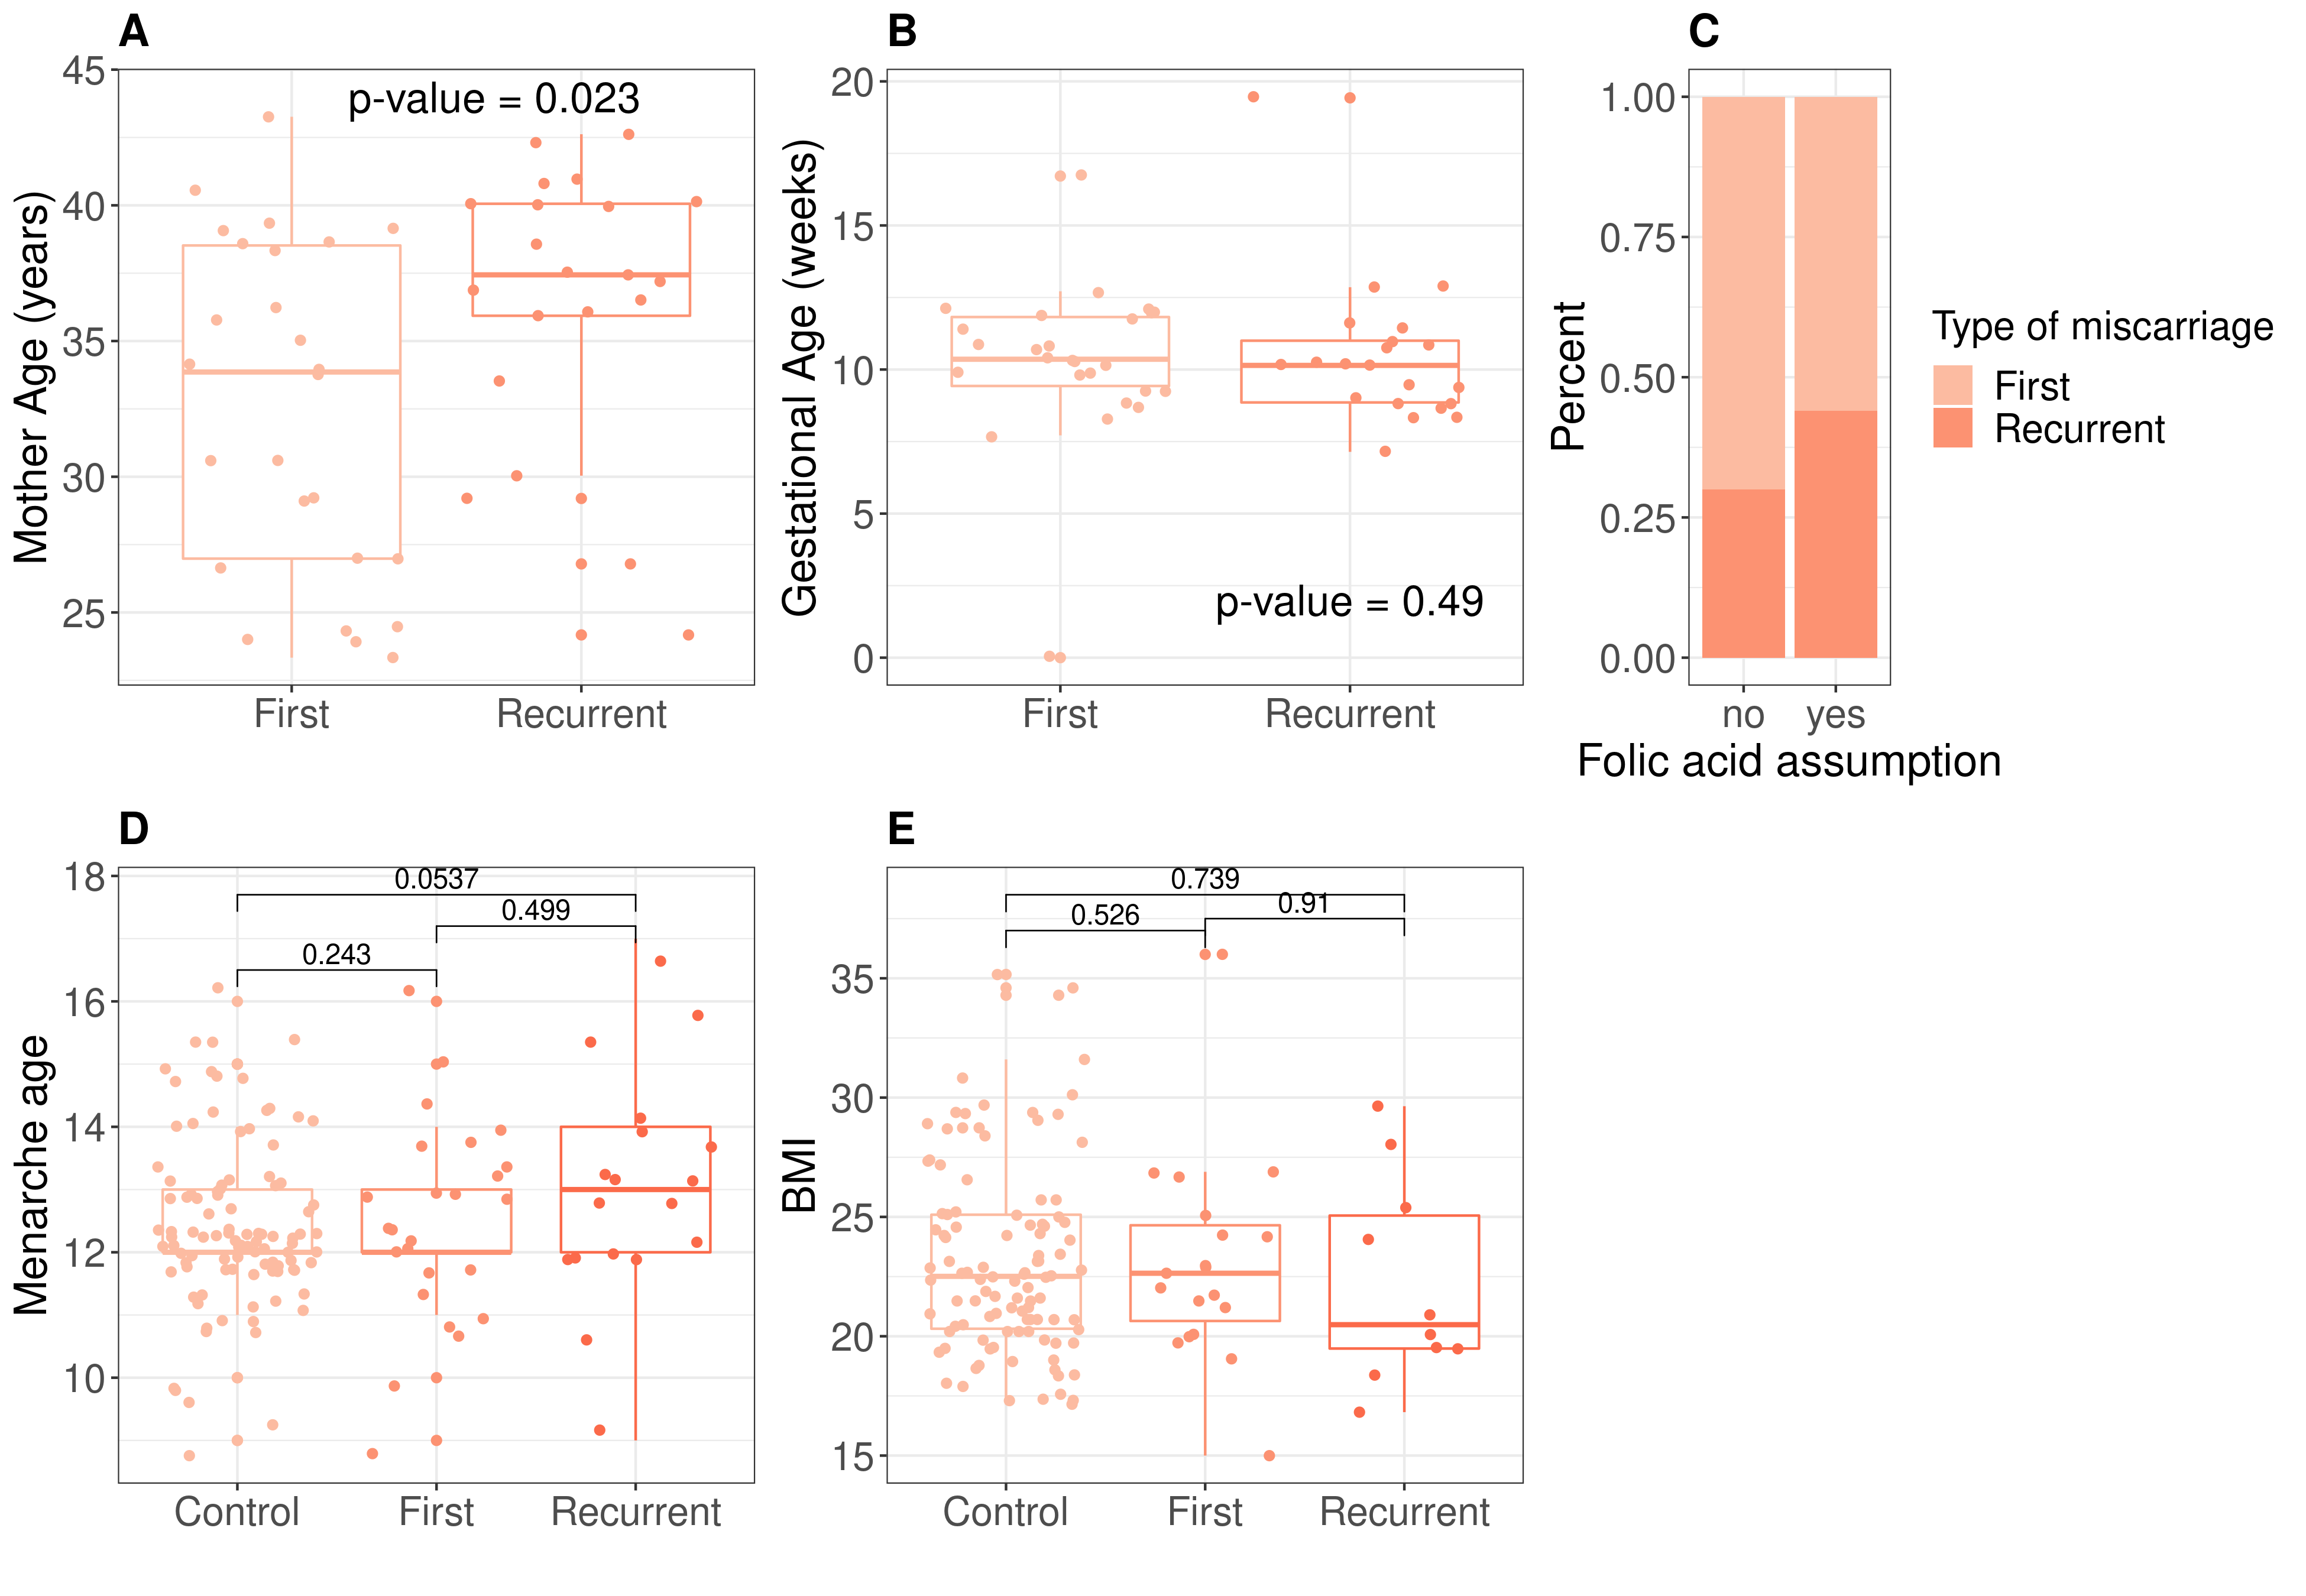
\includegraphics[width=\linewidth]{fig/panel_stats.png}
\caption{\textbf{Features of the embryo's mothers.} \textbf{(A)} Median age of the mother at the event is XX and XX for first and recurrent miscarriages, with no significant difference. \textbf{(B)} Gestational age at the time of the pregnancy termination range from X to X weeks with no significant difference between first and recurrent cases.  \textbf{(C)} Folic acid intake. Range of values of menarche age \textbf{(D)} and Body Mass Index \textbf{(E)} in embryo's mothers are not significantly different from a control set of mothers undergoing voluntary termination of pregnancy.}
\label{fig:embryostats}
\end{figure}

\begin{figure}[h]
\centering
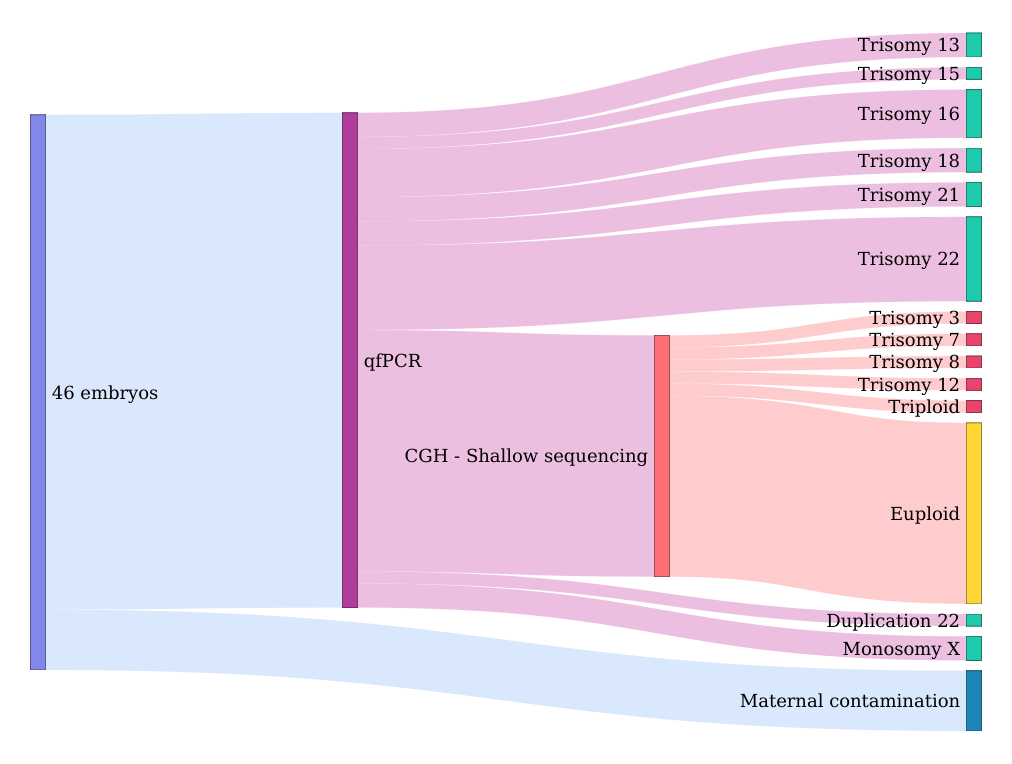
\includegraphics[width=0.7\textwidth]{fig/ibelieve.png}
\caption{\textbf{Outcome of the screening for aneuploidies in the embryos.} Screening on embryonic DNA by quantitative PCR, comparative hybridization and shallow sequencing finds aneuploidies in  56.6\% of the embryos, the most common being the trisomy of chromosome 22. In yellow the fraction of euploid embryos. }
\label{fig:presequencing}
\end{figure}

\begin{figure}[ht]
\centering
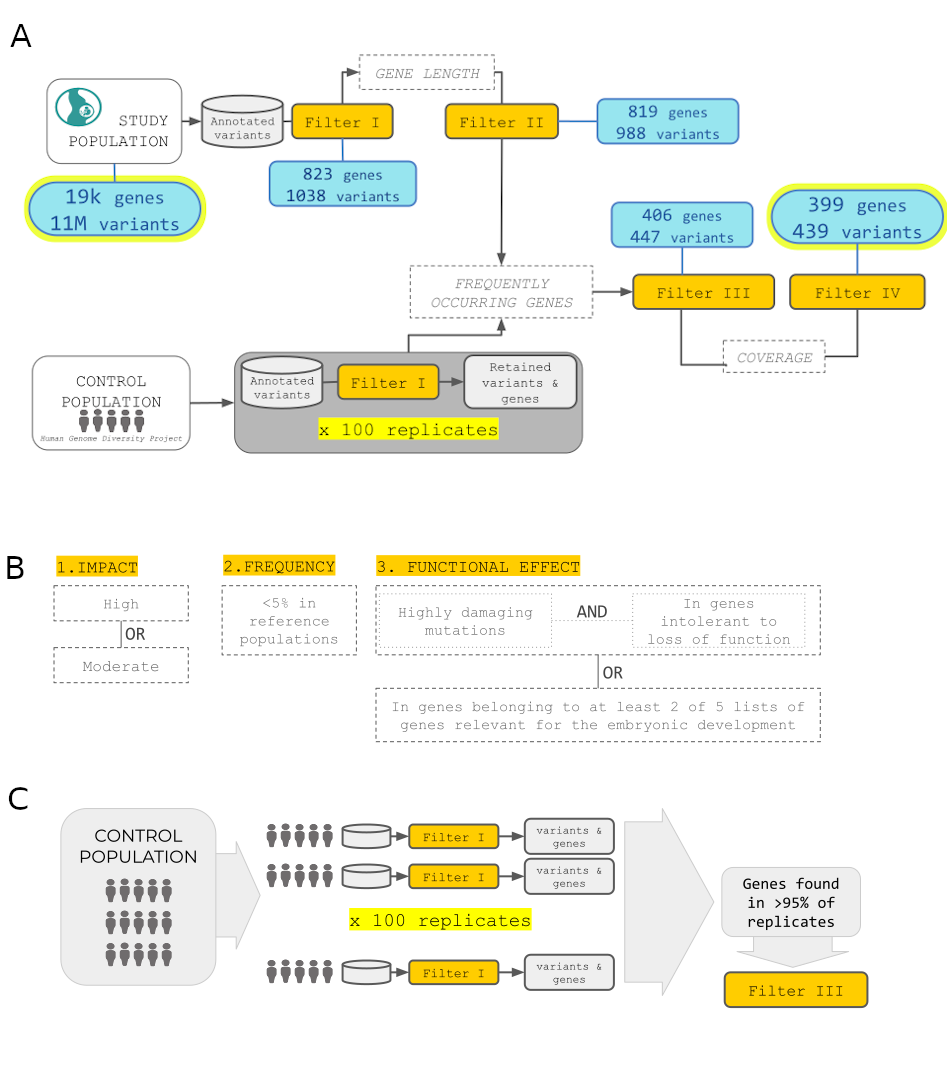
\includegraphics[width=\linewidth]{fig/pipe.png}
\caption{\textbf{Overview of the pipeline for prioritization of the genetic variants.} more text here } 
\label{fig:pipeline}
\end{figure}
%Genetic variants discovered in samples and controls are annotated and Filtered on the basis of the annotations (Filter I). In samples  Samples are first screened for the quality of DNA and maternal contamination and then analyzed for aneuploidies. \textbf{(B) Outcomes of the pipeline.} We estimate that 18\% of samples goes to sequencing....


\begin{figure}[ht]
\centering
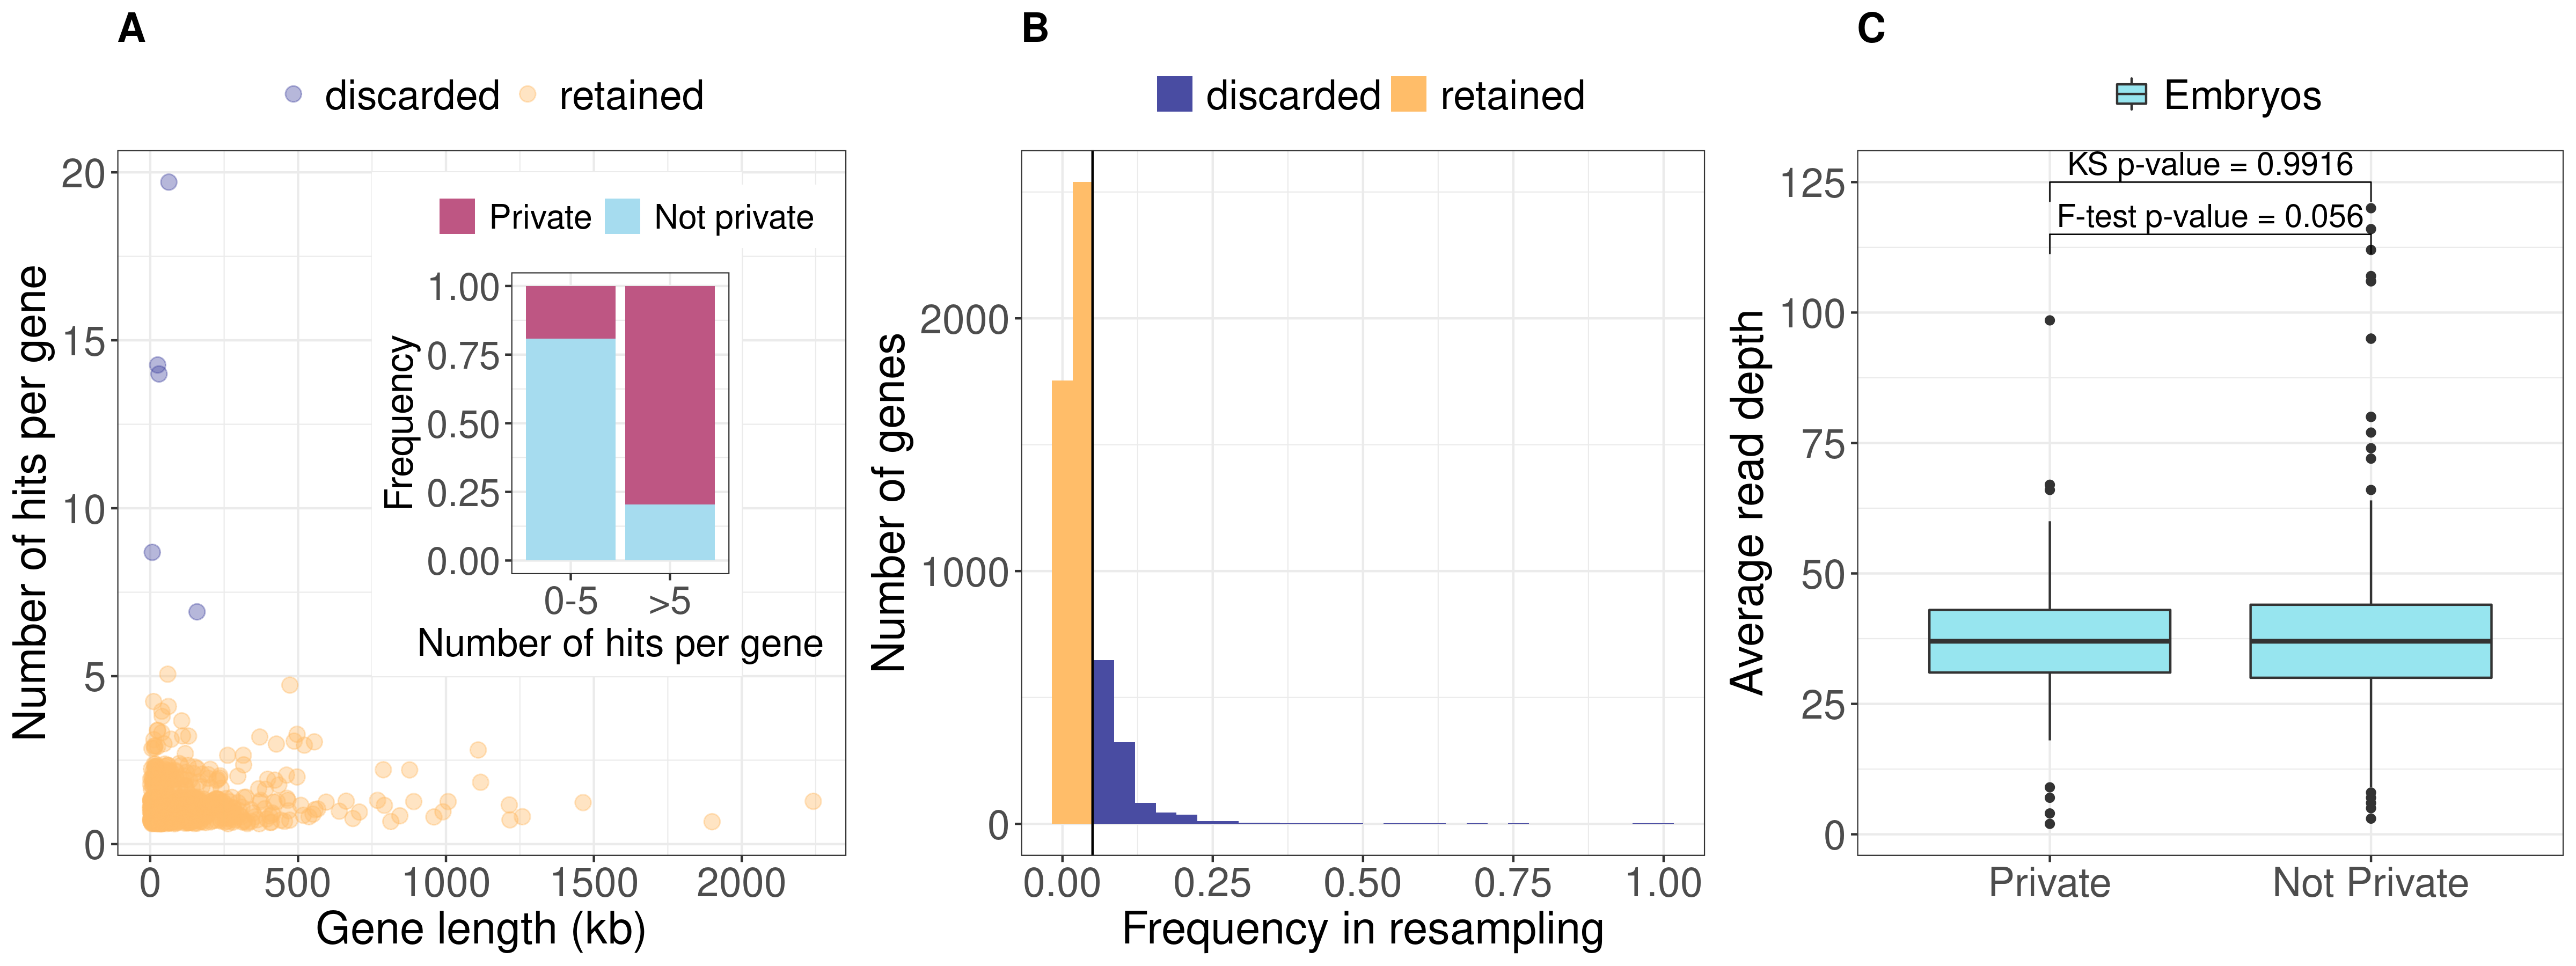
\includegraphics[width=\linewidth]{fig/filters_embryos.png}
\caption{\textbf{}}
\label{fig:filters}
\end{figure}

\begin{figure}[ht]
\centering
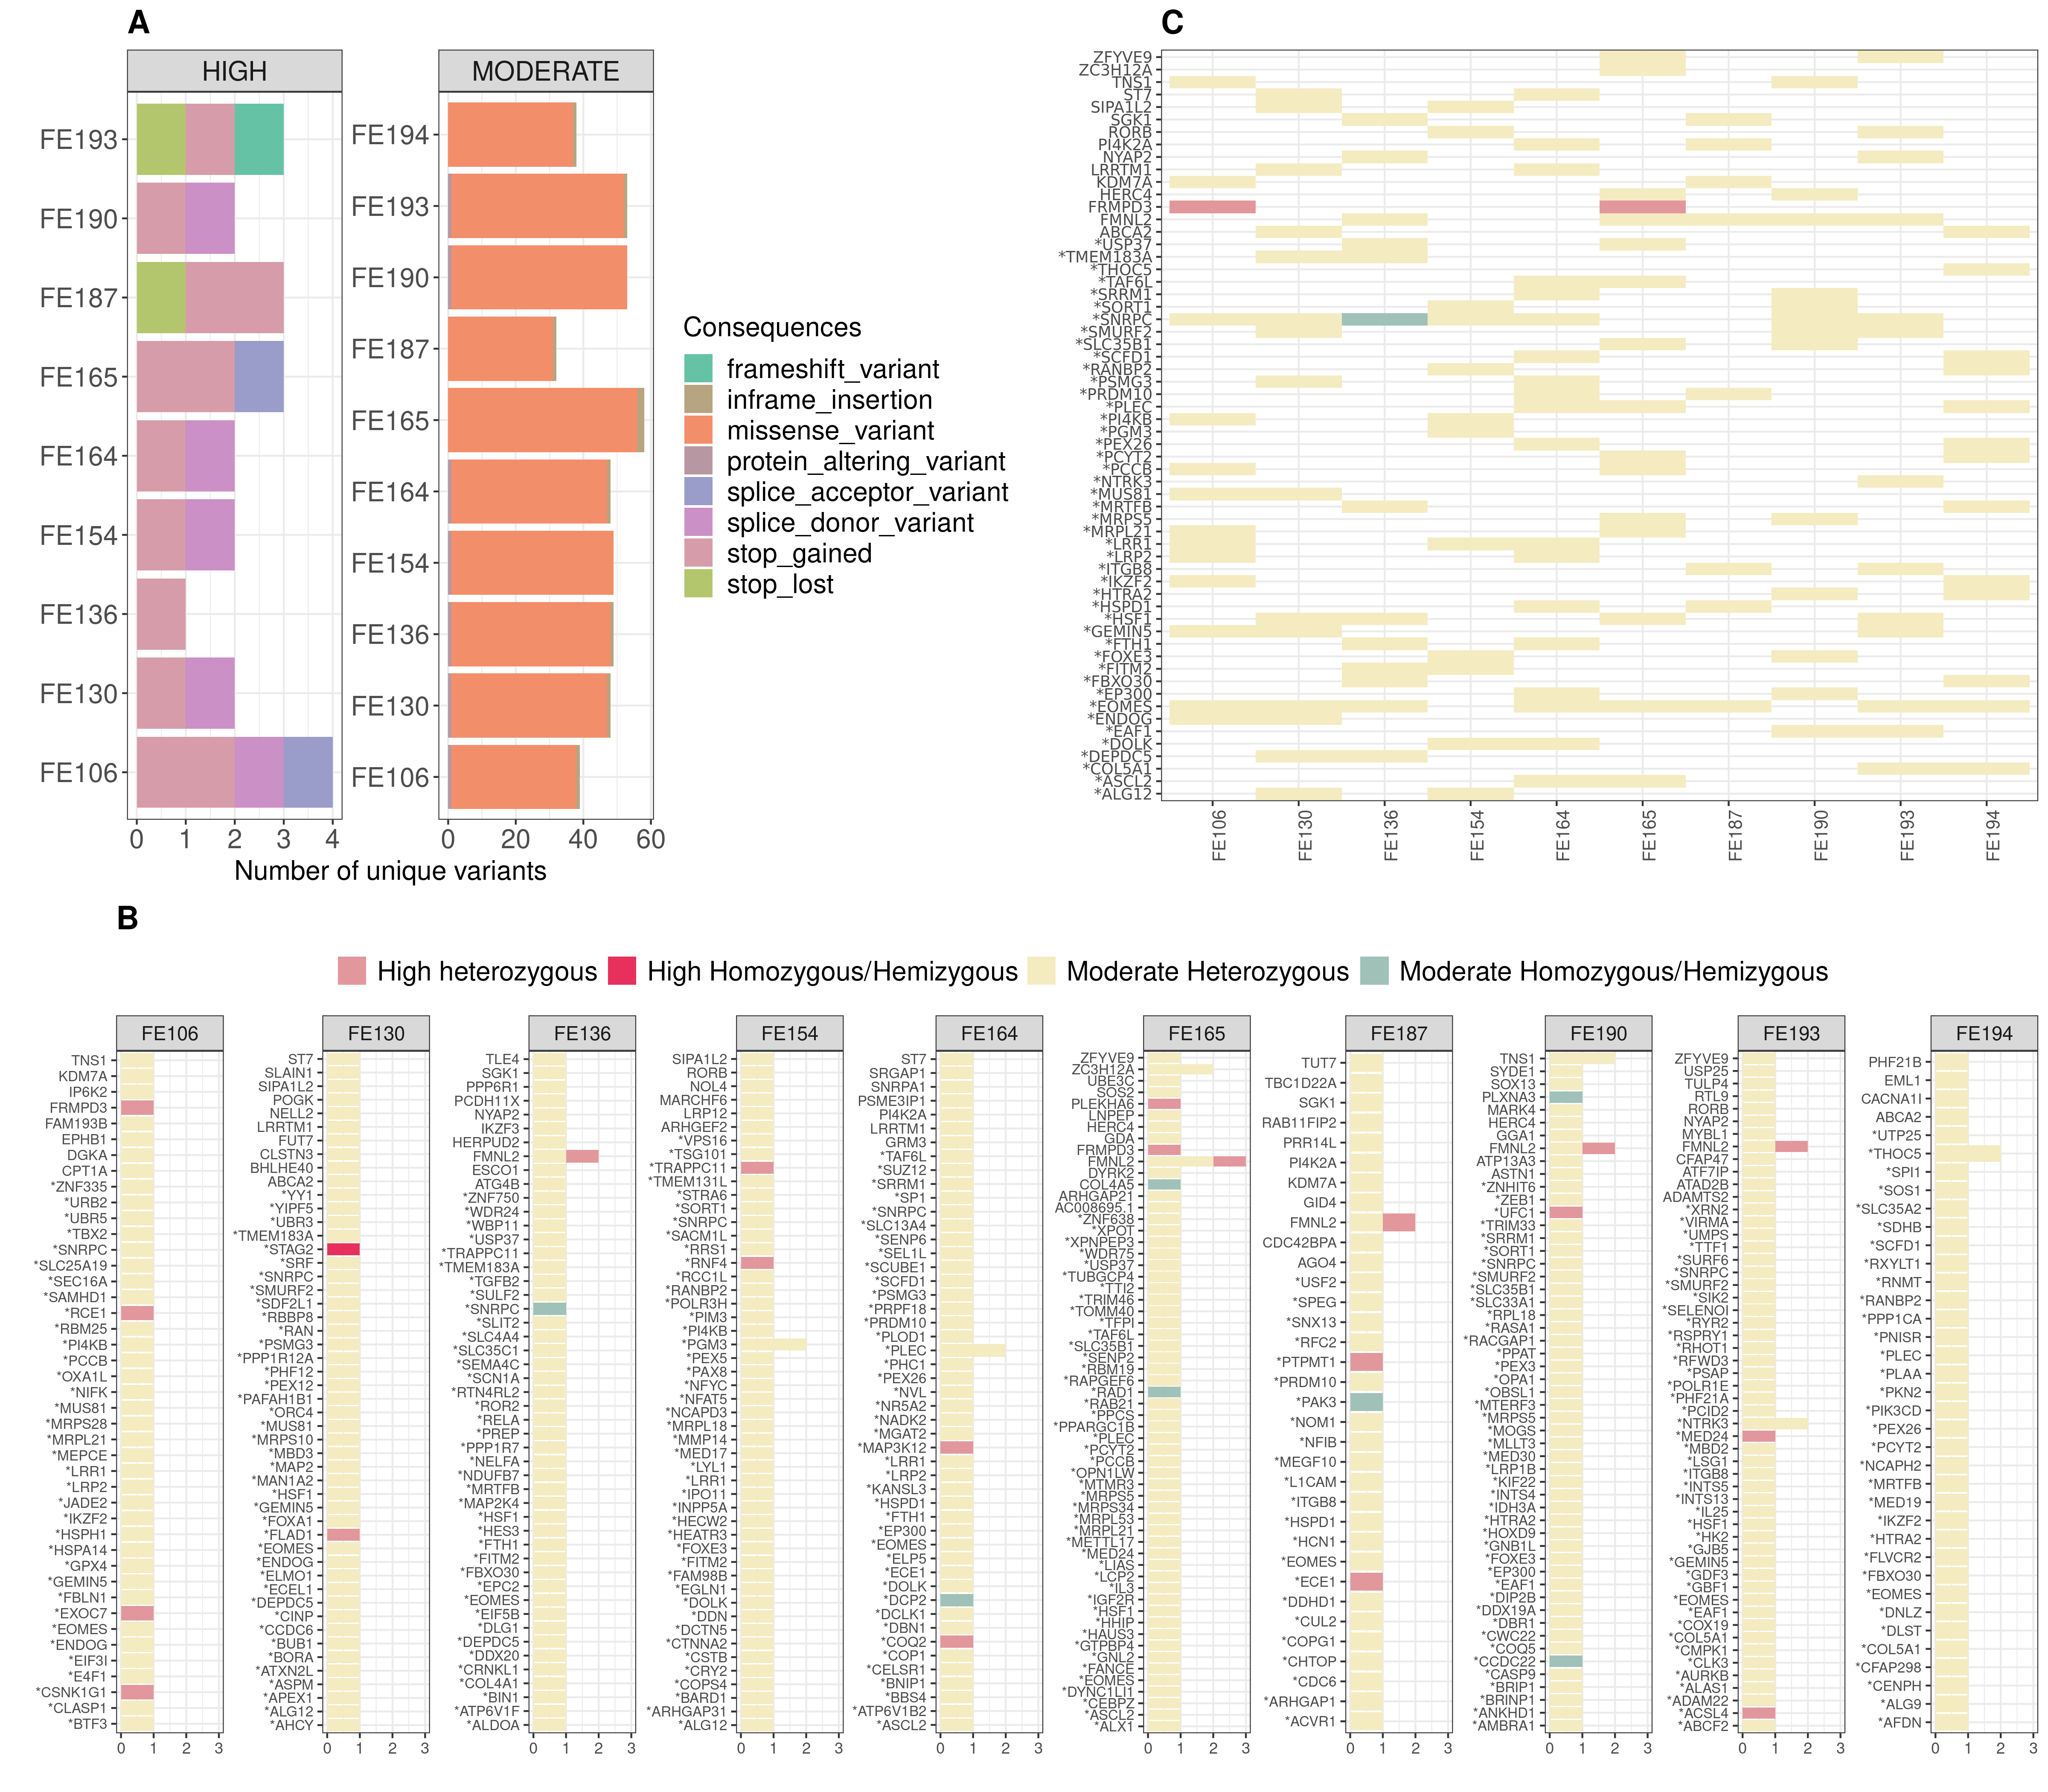
\includegraphics[width=\linewidth]{fig/panel_EmbryoResults.png}
%\caption{\textbf{} he occurrence of variants, their impact, and the count of the consequence allele per gene per embryo  }
\caption{\textbf{}}
\label{fig:resembryo}
\end{figure}

\begin{figure}[ht]
\centering
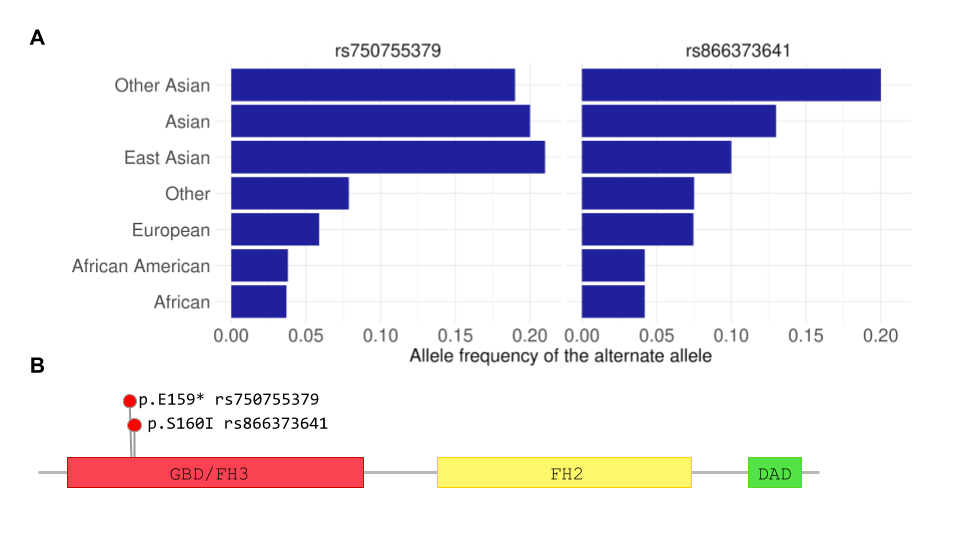
\includegraphics[width=\linewidth]{fig/fmnl2.png}
%\caption{\textbf{} he occurrence of variants, their impact, and the count of the consequence allele per gene per embryo  }
\caption{\textbf{}}
\label{fig:fmnl2}
\end{figure}


\beginsupplement
\section*{Supplementary Information}
%%%%%%%%%%%%%%%%%%%%%%%%%
%\subsection*{Supplementary Tables}
%\include{supptables}
%%%%%%%%%%%%%%%%%%%%%%%%%%
\subsection*{Supplementary Figures}
\begin{figure}[ht]
    \centering
    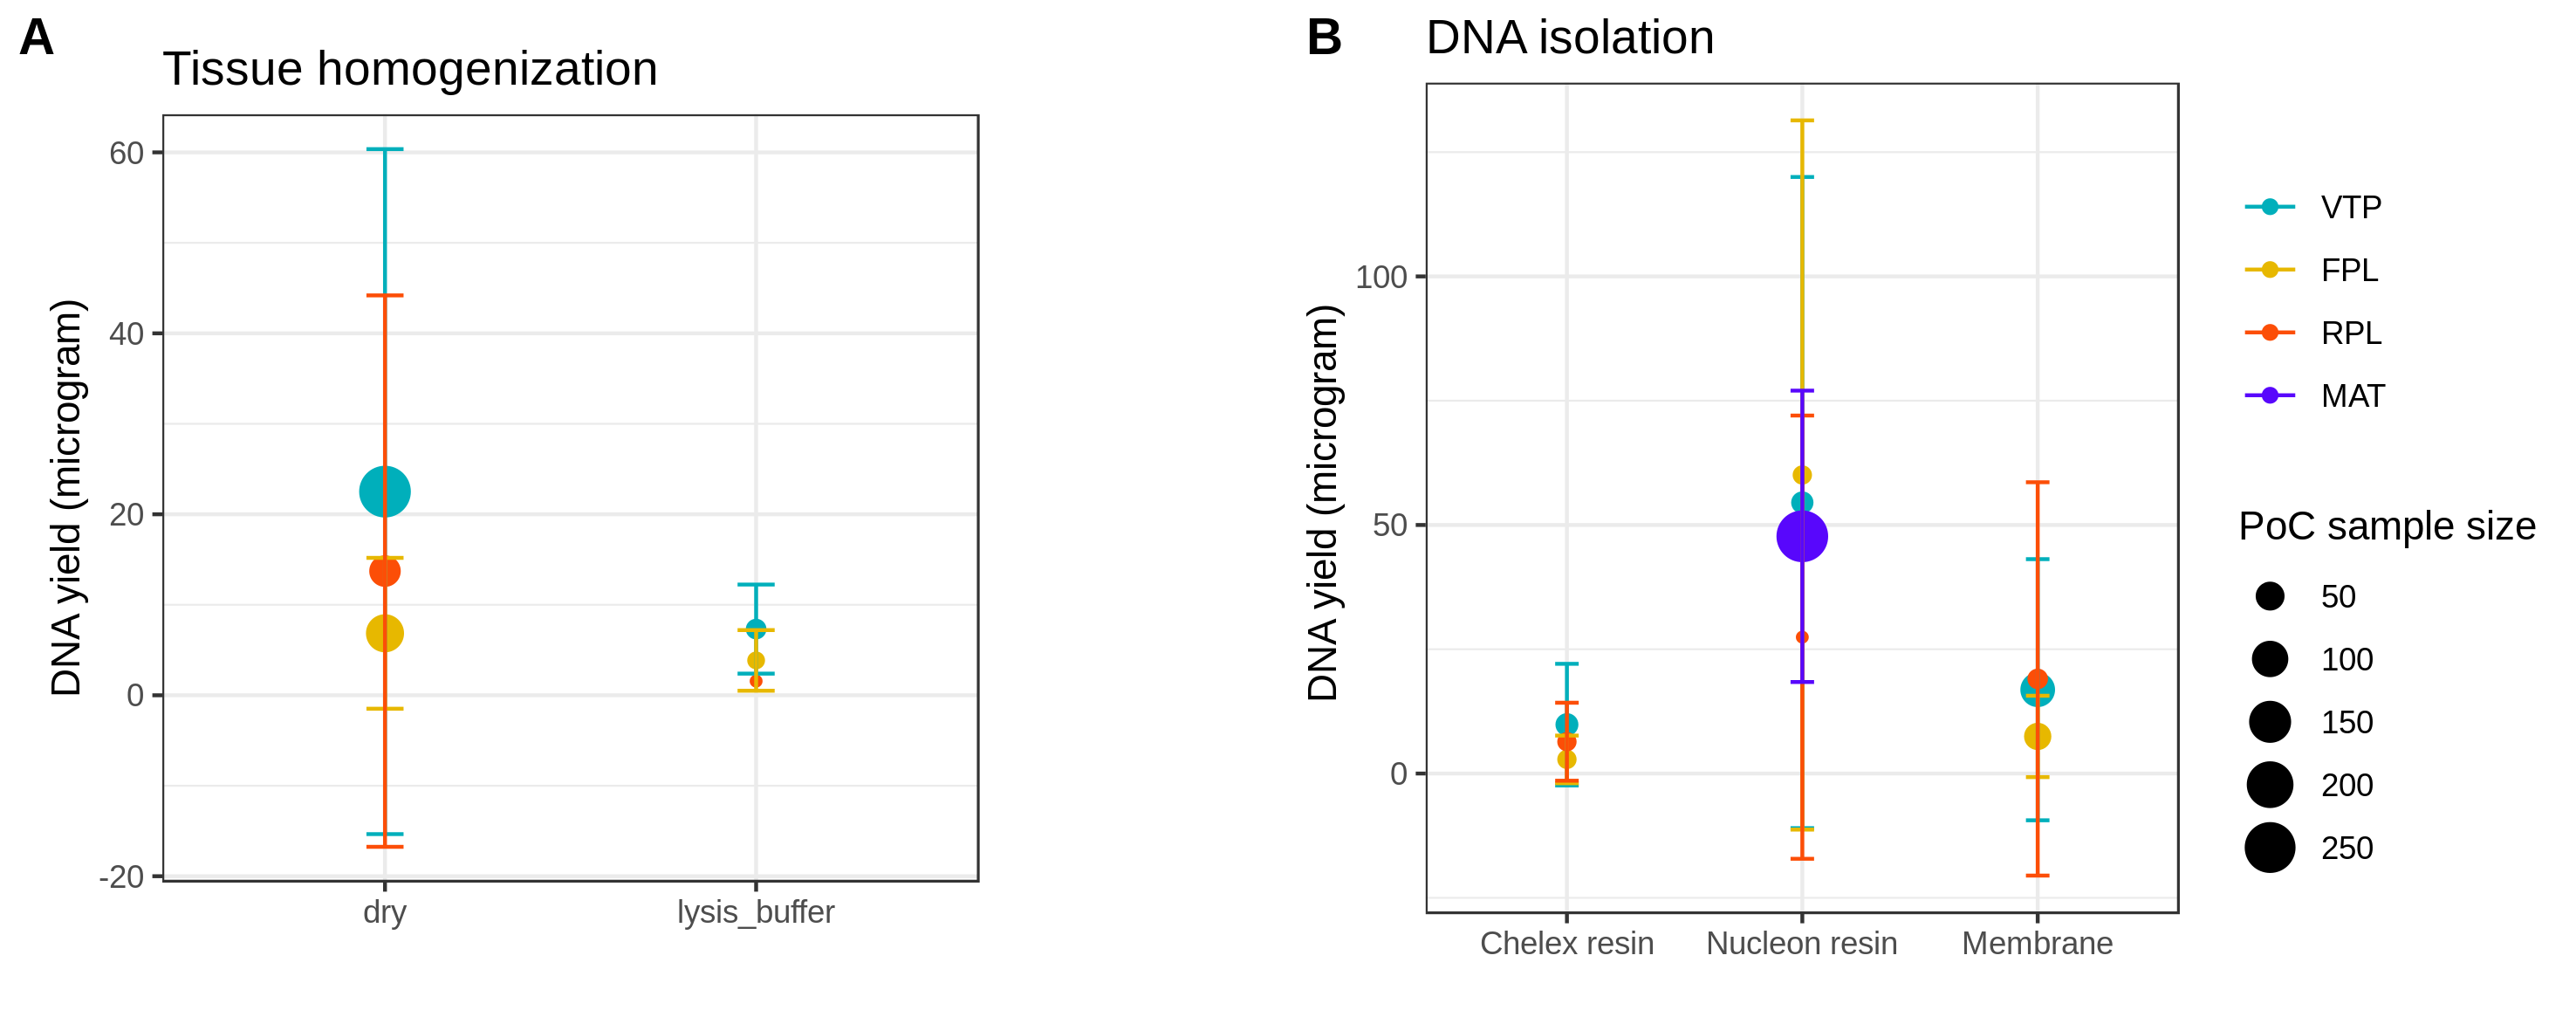
\includegraphics[width= 14 cm, high= 16cm]{fig/panelDNA.png}
    \caption{\textbf{Optimization of tissue homogenization and DNA extraction.} We do not observe significant difference between two methods of tissue homogenization (\textbf{A}), and three methods of DNA isolation (\textbf{b}) apart form a slightly higher range of yield for one type of resin. VTP: voluntary pregnancy termination;  FPL: first pregnancy loss; RPL:recurrent pregnancy loss;  MAT: maternal bllod; PoC: product of conception.}
    \label{fig:dna}
\end{figure}


%\begin{figure}[ht]
%    \centering
%    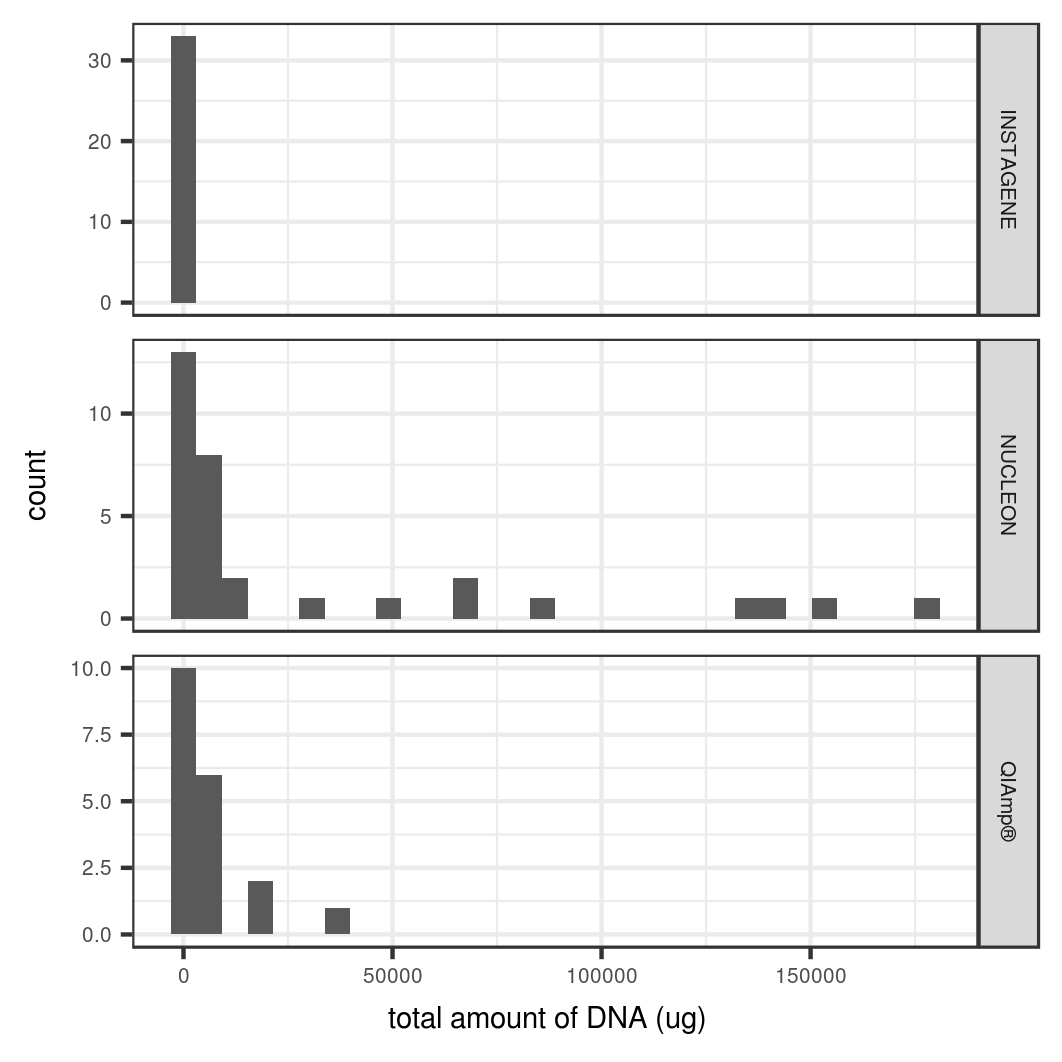
\includegraphics[width= 14 cm, high= 16cm]{fig/totaldna_bykit.png}
%    \caption{\textbf{Yeld of DNA extraction form chorionic villi by extraction kit.} Distributions of total DNA as quantified using the  Qubit 2.0 Fluorometer} 
%    \label{fig:dnayeld}
%\end{figure}


\begin{figure}[ht]
    \centering
    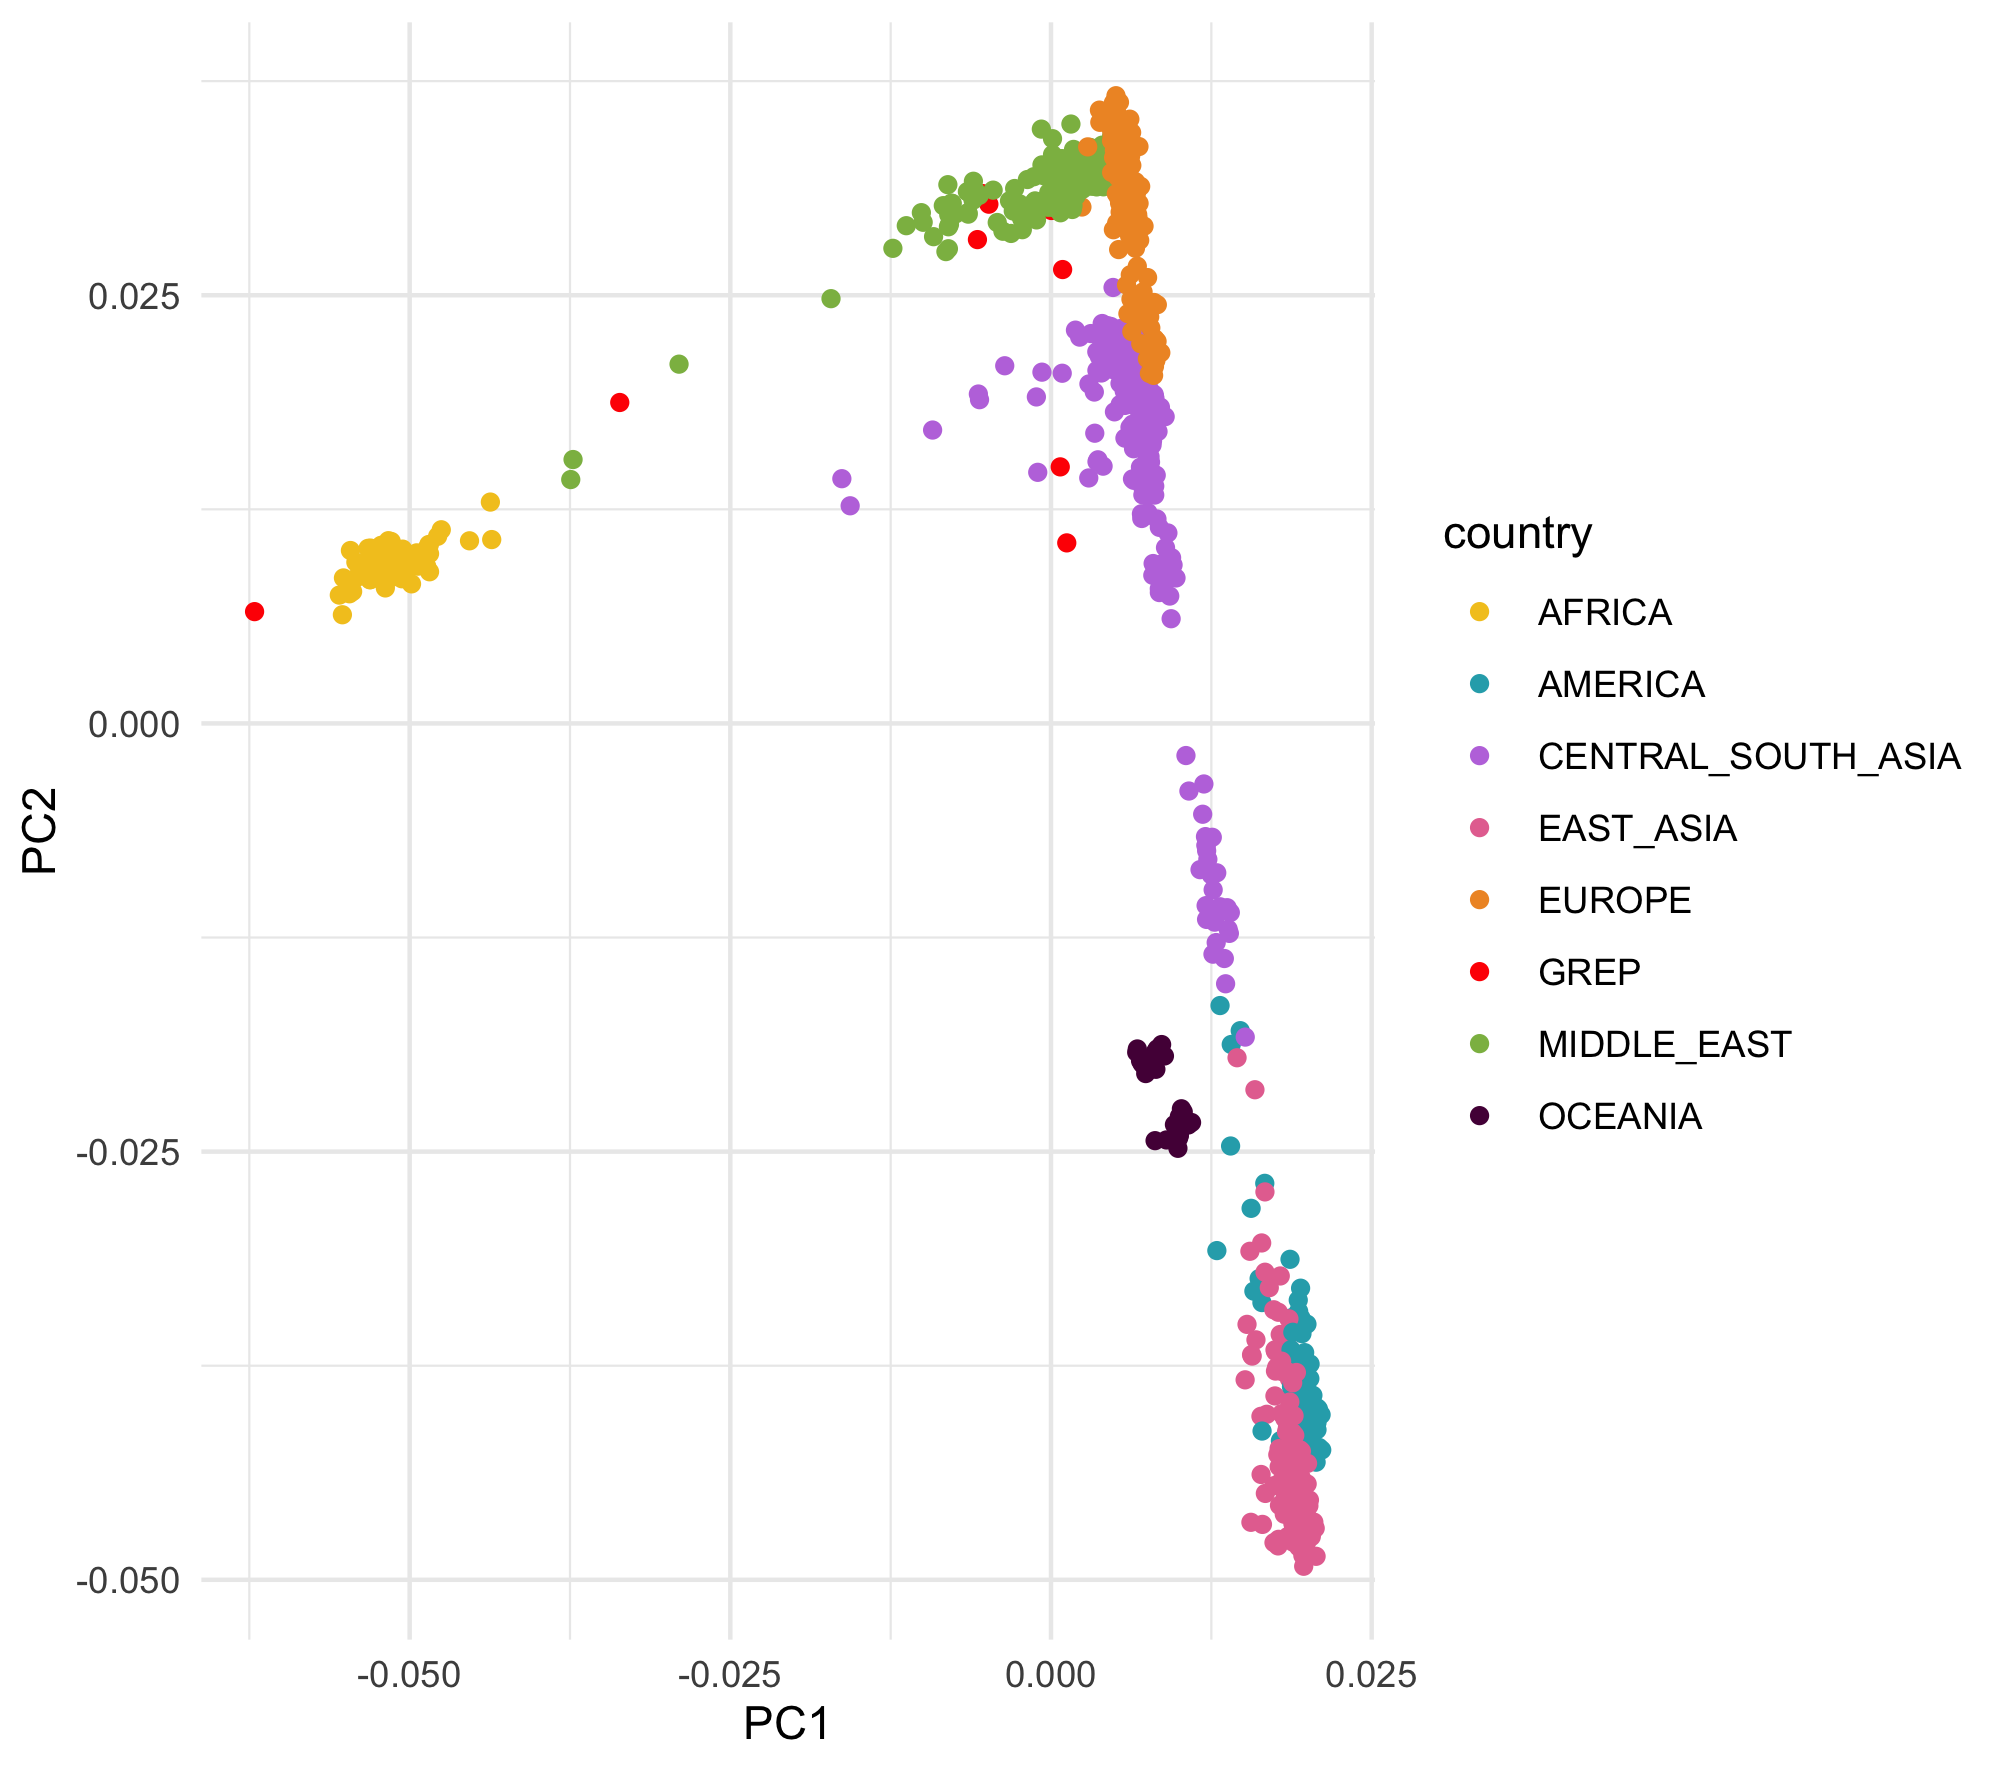
\includegraphics[width= 14 cm, high= 16cm]{fig/pca_hgdp-grep_noALPHA.png}
    \caption{\textbf{Principal Component Analysis.} Plot of the first and second components obtained using 1,2M autosomal SNPs and considering genomic data of the ten embryos sequenced in this study and publicly available data of individuals form the Human Genome Diversity Project}
    \label{fig:pca}
\end{figure}


\begin{figure}[ht]
    \centering
    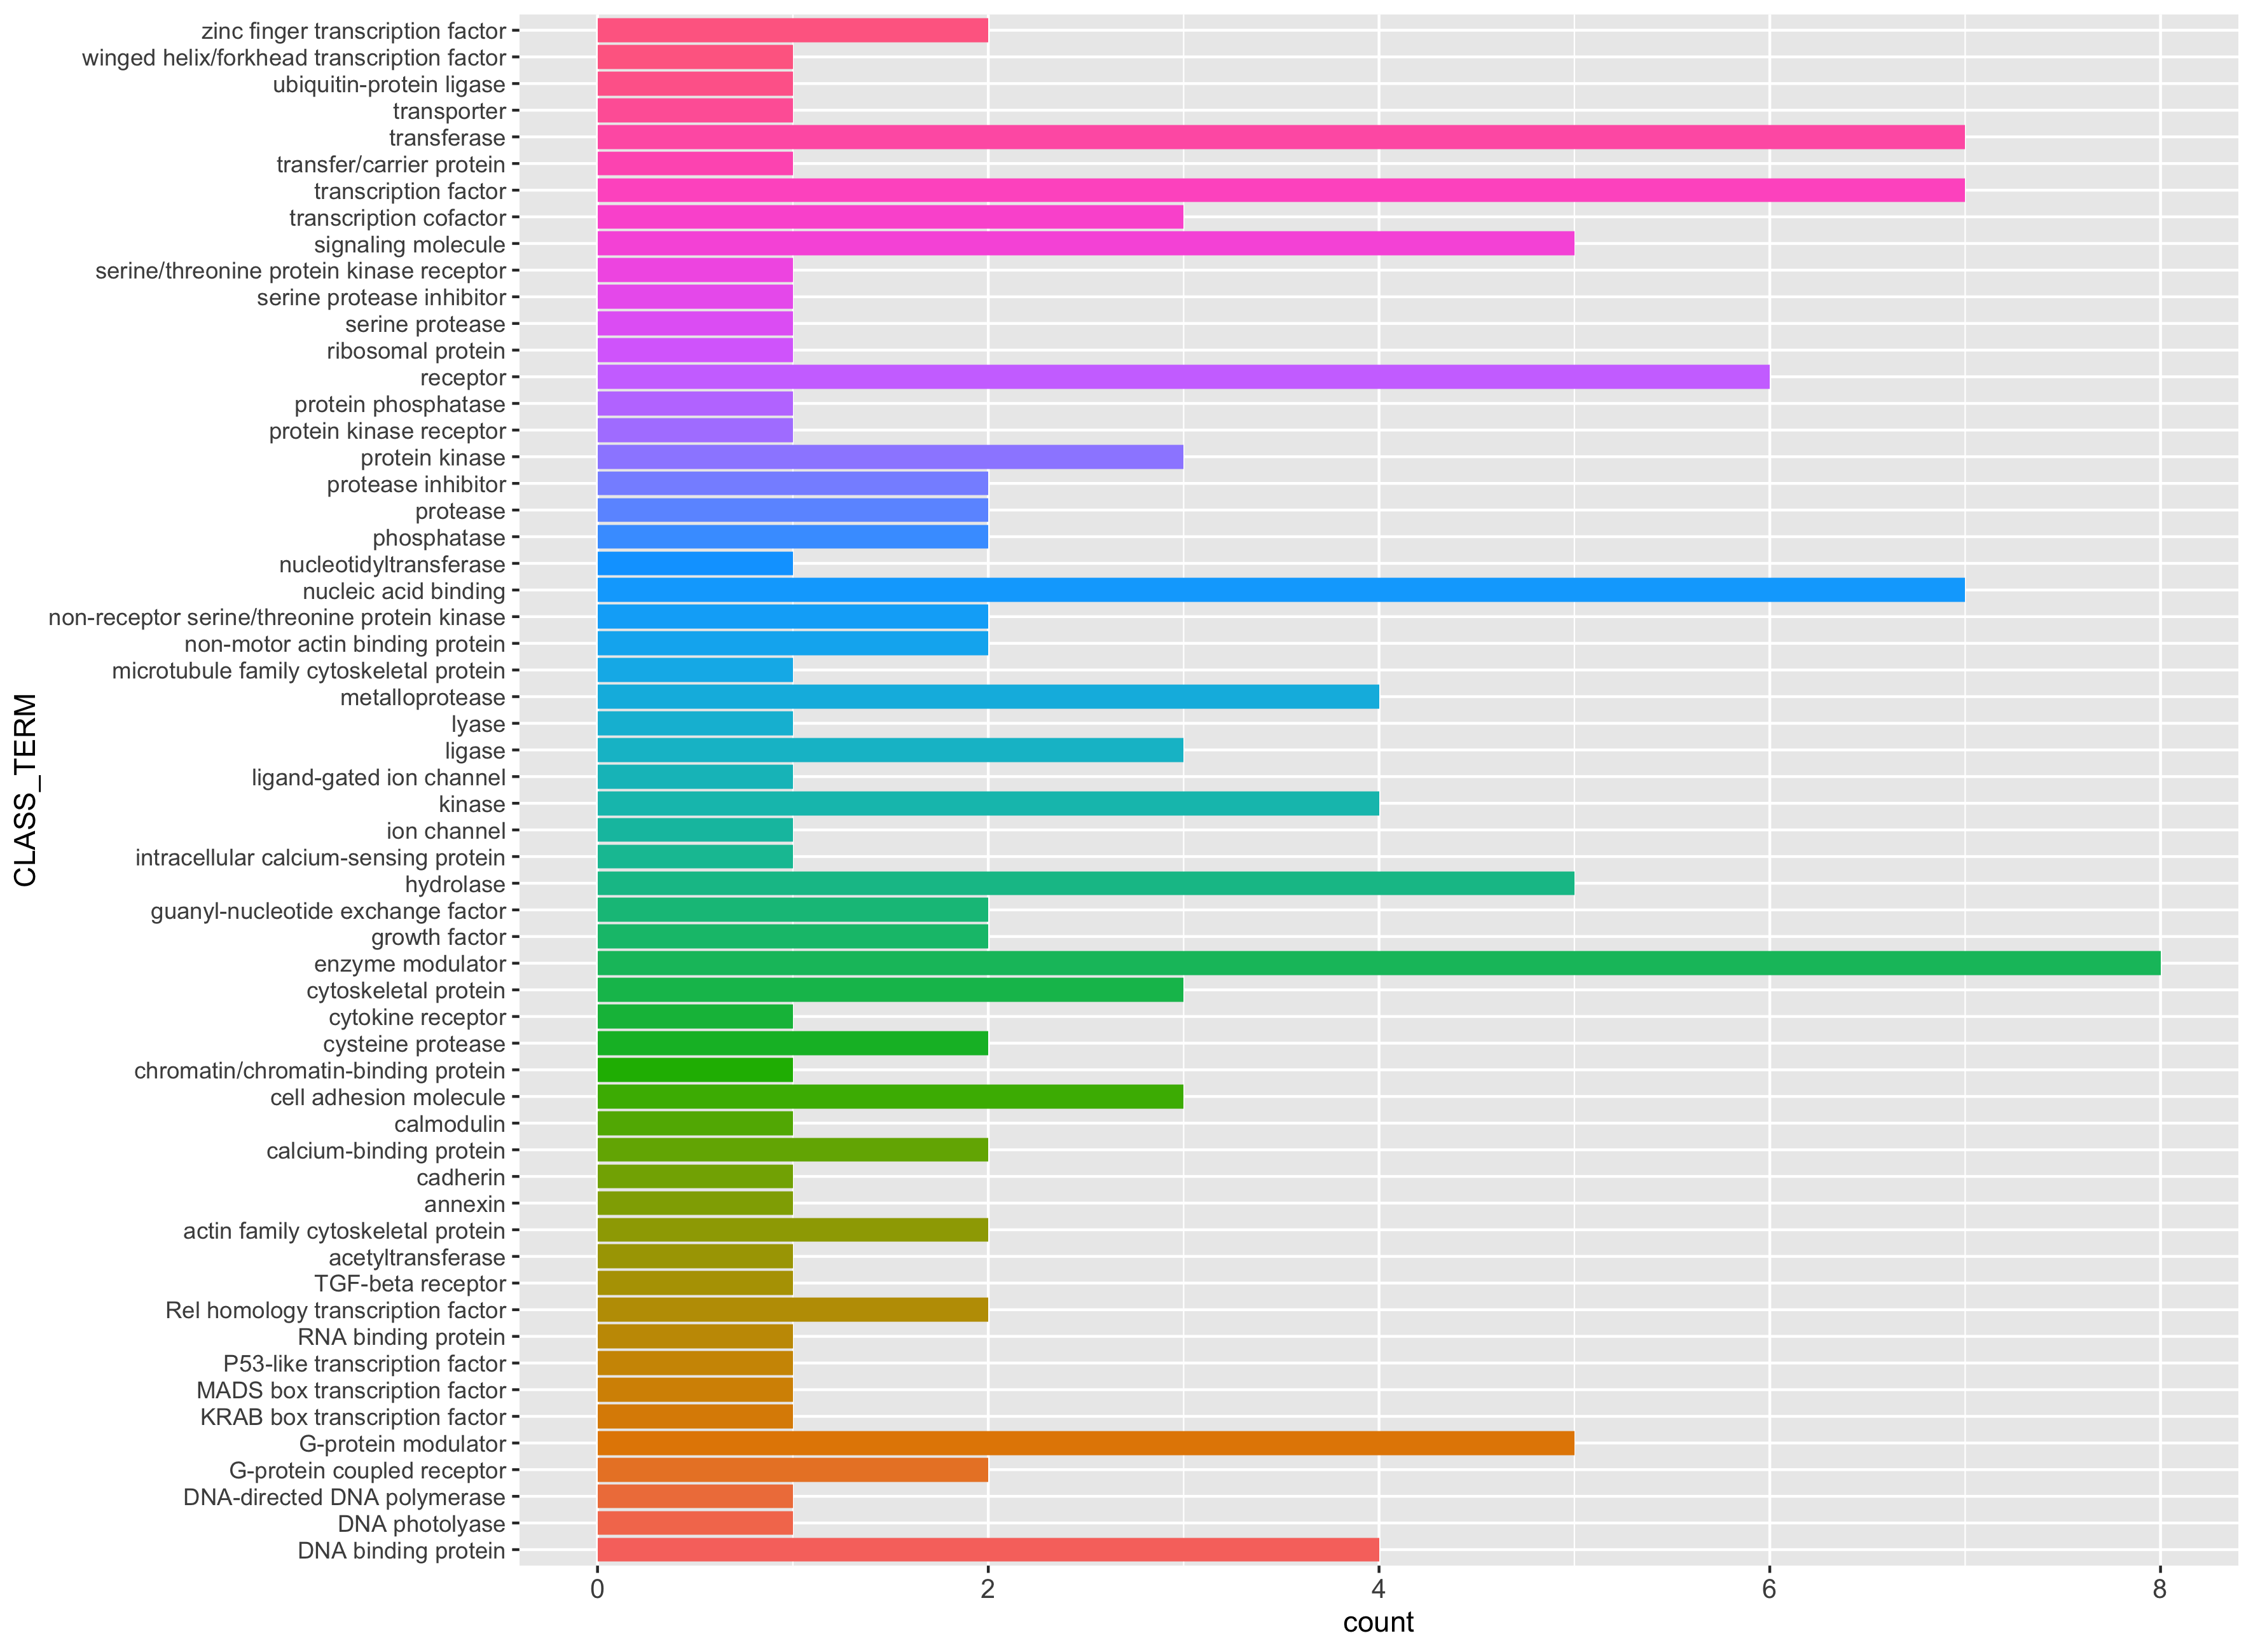
\includegraphics[width= 14 cm, high= 16cm]{fig/class_term_grep.png}
    \caption{\textbf{Classification of the prioritized genes by protein class. }}
    \label{fig:protClass}
\end{figure}




%\begin{figure}[ht]
%    \centering
%    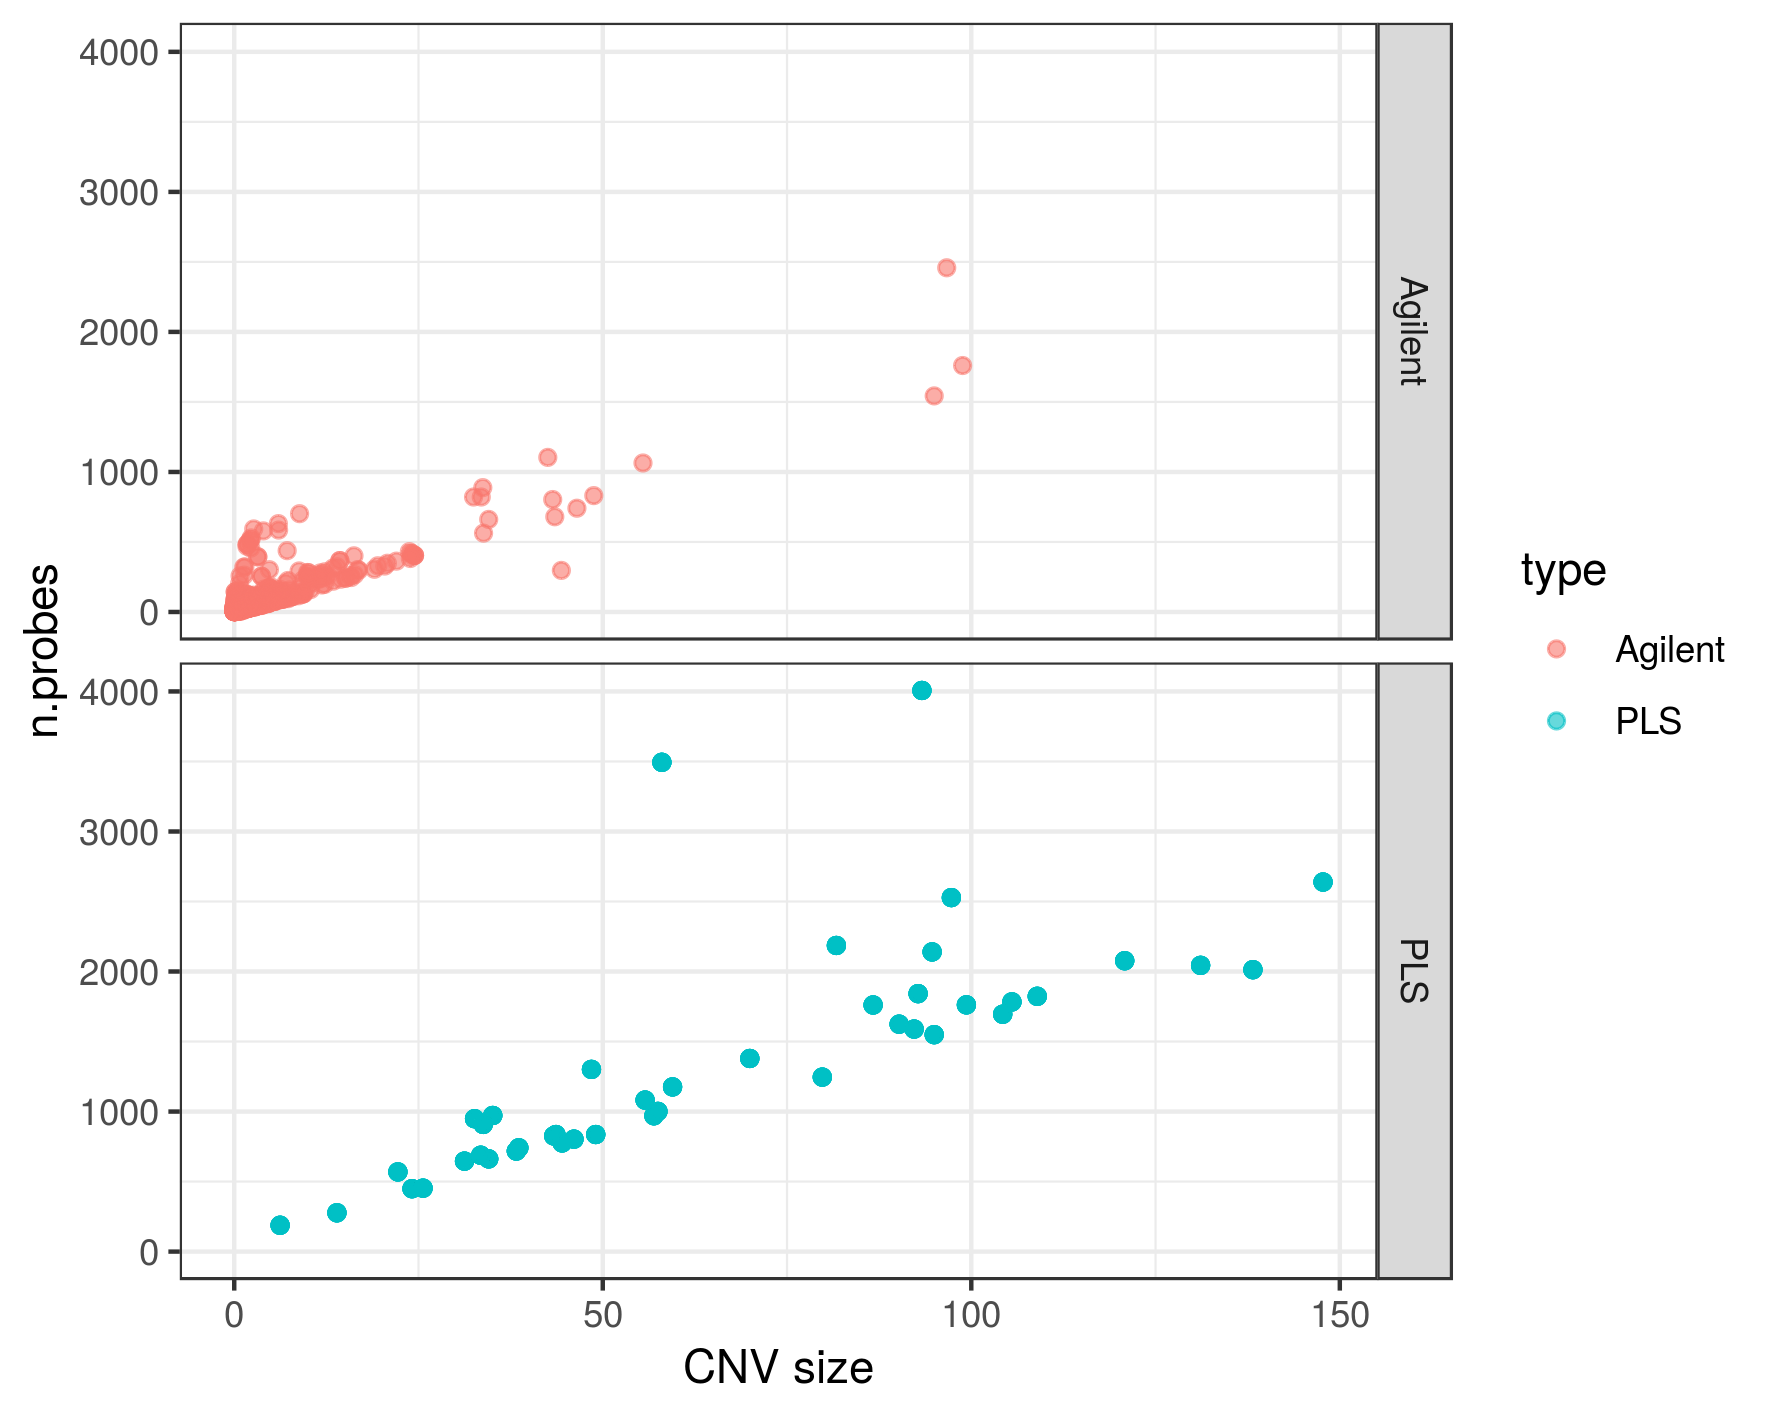
\includegraphics[width= 14 cm, high= 16cm]{fig/cnvCallComparison.png}
%    \caption{\textbf{Copy number variant detection.} Comparison of calls made by the Agilent software and the penalized least square method implemented in the copynumber R package \cite{nilsen2012copynumber}} 
%    \label{fig:cnvmethods}
%\end{figure}
%\begin{landscape}
\begin{table}[]
\resizebox{\textwidth}{!}{%
\begin{tabular}{|l|l|l|l|l|l|l|}
\hline
{\color[HTML]{000000} \textbf{ID}} & \textbf{origin} & \textbf{Full term births} & \textbf{Previous miscarriages} & \textbf{Induced abortion} & \textbf{Preterm birth} & \textbf{type of miscarriage} \\ \hline
{\color[HTML]{000000} AS006}       & European        & 0                         & 0                              & 0                         & 0                      & miscarriage first            \\ \hline
{\color[HTML]{000000} AS030}       & European        & 1                         & 1                              & 0                         & 0                      & miscarriage first            \\ \hline
AS036                              & European        & 0                         & 0                              & 0                         & 0                      & miscarriage first            \\ \hline
AS054                              & African         & 1                         & 0                              & 2                         & 0                      & miscarriage first            \\ \hline
AS064                              & European        & 0                         & 0                              & 0                         & 0                      & miscarriage\_first           \\ \hline
AS065                              & European        & 0                         & 0                              & 0                         & 0                      & miscarriage first            \\ \hline
AS087                              & Asian           & 0                         & 3                              & 0                         & 1                      & miscarriage recurrent        \\ \hline
AS090                              & European        & 1                         & 0                              & 0                         & 0                      & miscarriage first            \\ \hline
AS093                              & Asian           & 0                         & 2                              & 0                         & 0                      & miscarriage recurrent        \\ \hline
AS094                              & European        & 3                         & 3                              & 0                         & 0                      & miscarriage recurrent        \\ \hline
\end{tabular}%
}
\caption{}
\label{tab:medicalfields}
\end{table}
\end{landscape}

\begin{landscape}
\begin{table}[]
\resizebox{\textwidth}{!}{%
\begin{tabular}{|l|l|l|l|l|}
\hline
\textbf{Gene symbol} & \textbf{Gene length (kb)} & \textbf{Nb. of paralogues (range identity)} & \textbf{hist in embryos} & \textbf{hits in women} \\ \hline
\textit{C2CD3}       & 7.96                      &                                             & 7                        & 0                      \\ \hline
\textit{FIGN}        & 9.5                       & 10 (24-41\%)                                & 16                       & 0                      \\ \hline
\textit{GXYLT1}      & 63                        &                                             & 20                       & 19                     \\ \hline
\textit{MTCH2}       & 29.8                      &                                             & 14                       & 12                     \\ \hline
\textit{MUC1}        & 7.09                      &                                             & 9                        & 9                      \\ \hline
\textit{MUC5B}       & 39.1                      &                                             & 0                        & 6                      \\ \hline
\textit{PCSK5}       & 472                       & 9 (11-52\%)                                 & 0                        & 6                      \\ \hline
\end{tabular}%
}
\caption{Caption}
\label{tab:paralogs}
\end{table}
\end{landscape}




\end{document}
